% Options for packages loaded elsewhere
\PassOptionsToPackage{unicode}{hyperref}
\PassOptionsToPackage{hyphens}{url}
%
\documentclass[
]{book}
\usepackage{amsmath,amssymb}
\usepackage{lmodern}
\usepackage{iftex}
\ifPDFTeX
  \usepackage[T1]{fontenc}
  \usepackage[utf8]{inputenc}
  \usepackage{textcomp} % provide euro and other symbols
\else % if luatex or xetex
  \usepackage{unicode-math}
  \defaultfontfeatures{Scale=MatchLowercase}
  \defaultfontfeatures[\rmfamily]{Ligatures=TeX,Scale=1}
\fi
% Use upquote if available, for straight quotes in verbatim environments
\IfFileExists{upquote.sty}{\usepackage{upquote}}{}
\IfFileExists{microtype.sty}{% use microtype if available
  \usepackage[]{microtype}
  \UseMicrotypeSet[protrusion]{basicmath} % disable protrusion for tt fonts
}{}
\makeatletter
\@ifundefined{KOMAClassName}{% if non-KOMA class
  \IfFileExists{parskip.sty}{%
    \usepackage{parskip}
  }{% else
    \setlength{\parindent}{0pt}
    \setlength{\parskip}{6pt plus 2pt minus 1pt}}
}{% if KOMA class
  \KOMAoptions{parskip=half}}
\makeatother
\usepackage{xcolor}
\IfFileExists{xurl.sty}{\usepackage{xurl}}{} % add URL line breaks if available
\IfFileExists{bookmark.sty}{\usepackage{bookmark}}{\usepackage{hyperref}}
\hypersetup{
  pdftitle={Demystifying Structural Equation Modeling},
  pdfauthor={Jonathan Amburgey and Sean Raleigh, Westminster College (Salt Lake City, UT)},
  hidelinks,
  pdfcreator={LaTeX via pandoc}}
\urlstyle{same} % disable monospaced font for URLs
\usepackage{color}
\usepackage{fancyvrb}
\newcommand{\VerbBar}{|}
\newcommand{\VERB}{\Verb[commandchars=\\\{\}]}
\DefineVerbatimEnvironment{Highlighting}{Verbatim}{commandchars=\\\{\}}
% Add ',fontsize=\small' for more characters per line
\usepackage{framed}
\definecolor{shadecolor}{RGB}{248,248,248}
\newenvironment{Shaded}{\begin{snugshade}}{\end{snugshade}}
\newcommand{\AlertTok}[1]{\textcolor[rgb]{0.94,0.16,0.16}{#1}}
\newcommand{\AnnotationTok}[1]{\textcolor[rgb]{0.56,0.35,0.01}{\textbf{\textit{#1}}}}
\newcommand{\AttributeTok}[1]{\textcolor[rgb]{0.77,0.63,0.00}{#1}}
\newcommand{\BaseNTok}[1]{\textcolor[rgb]{0.00,0.00,0.81}{#1}}
\newcommand{\BuiltInTok}[1]{#1}
\newcommand{\CharTok}[1]{\textcolor[rgb]{0.31,0.60,0.02}{#1}}
\newcommand{\CommentTok}[1]{\textcolor[rgb]{0.56,0.35,0.01}{\textit{#1}}}
\newcommand{\CommentVarTok}[1]{\textcolor[rgb]{0.56,0.35,0.01}{\textbf{\textit{#1}}}}
\newcommand{\ConstantTok}[1]{\textcolor[rgb]{0.00,0.00,0.00}{#1}}
\newcommand{\ControlFlowTok}[1]{\textcolor[rgb]{0.13,0.29,0.53}{\textbf{#1}}}
\newcommand{\DataTypeTok}[1]{\textcolor[rgb]{0.13,0.29,0.53}{#1}}
\newcommand{\DecValTok}[1]{\textcolor[rgb]{0.00,0.00,0.81}{#1}}
\newcommand{\DocumentationTok}[1]{\textcolor[rgb]{0.56,0.35,0.01}{\textbf{\textit{#1}}}}
\newcommand{\ErrorTok}[1]{\textcolor[rgb]{0.64,0.00,0.00}{\textbf{#1}}}
\newcommand{\ExtensionTok}[1]{#1}
\newcommand{\FloatTok}[1]{\textcolor[rgb]{0.00,0.00,0.81}{#1}}
\newcommand{\FunctionTok}[1]{\textcolor[rgb]{0.00,0.00,0.00}{#1}}
\newcommand{\ImportTok}[1]{#1}
\newcommand{\InformationTok}[1]{\textcolor[rgb]{0.56,0.35,0.01}{\textbf{\textit{#1}}}}
\newcommand{\KeywordTok}[1]{\textcolor[rgb]{0.13,0.29,0.53}{\textbf{#1}}}
\newcommand{\NormalTok}[1]{#1}
\newcommand{\OperatorTok}[1]{\textcolor[rgb]{0.81,0.36,0.00}{\textbf{#1}}}
\newcommand{\OtherTok}[1]{\textcolor[rgb]{0.56,0.35,0.01}{#1}}
\newcommand{\PreprocessorTok}[1]{\textcolor[rgb]{0.56,0.35,0.01}{\textit{#1}}}
\newcommand{\RegionMarkerTok}[1]{#1}
\newcommand{\SpecialCharTok}[1]{\textcolor[rgb]{0.00,0.00,0.00}{#1}}
\newcommand{\SpecialStringTok}[1]{\textcolor[rgb]{0.31,0.60,0.02}{#1}}
\newcommand{\StringTok}[1]{\textcolor[rgb]{0.31,0.60,0.02}{#1}}
\newcommand{\VariableTok}[1]{\textcolor[rgb]{0.00,0.00,0.00}{#1}}
\newcommand{\VerbatimStringTok}[1]{\textcolor[rgb]{0.31,0.60,0.02}{#1}}
\newcommand{\WarningTok}[1]{\textcolor[rgb]{0.56,0.35,0.01}{\textbf{\textit{#1}}}}
\usepackage{longtable,booktabs,array}
\usepackage{calc} % for calculating minipage widths
% Correct order of tables after \paragraph or \subparagraph
\usepackage{etoolbox}
\makeatletter
\patchcmd\longtable{\par}{\if@noskipsec\mbox{}\fi\par}{}{}
\makeatother
% Allow footnotes in longtable head/foot
\IfFileExists{footnotehyper.sty}{\usepackage{footnotehyper}}{\usepackage{footnote}}
\makesavenoteenv{longtable}
\usepackage{graphicx}
\makeatletter
\def\maxwidth{\ifdim\Gin@nat@width>\linewidth\linewidth\else\Gin@nat@width\fi}
\def\maxheight{\ifdim\Gin@nat@height>\textheight\textheight\else\Gin@nat@height\fi}
\makeatother
% Scale images if necessary, so that they will not overflow the page
% margins by default, and it is still possible to overwrite the defaults
% using explicit options in \includegraphics[width, height, ...]{}
\setkeys{Gin}{width=\maxwidth,height=\maxheight,keepaspectratio}
% Set default figure placement to htbp
\makeatletter
\def\fps@figure{htbp}
\makeatother
\setlength{\emergencystretch}{3em} % prevent overfull lines
\providecommand{\tightlist}{%
  \setlength{\itemsep}{0pt}\setlength{\parskip}{0pt}}
\setcounter{secnumdepth}{5}
\usepackage{booktabs}
\usepackage{amsthm}
\makeatletter
\def\thm@space@setup{%
  \thm@preskip=8pt plus 2pt minus 4pt
  \thm@postskip=\thm@preskip
}
\makeatother
\ifLuaTeX
  \usepackage{selnolig}  % disable illegal ligatures
\fi
\usepackage[]{natbib}
\bibliographystyle{apalike}

\title{Demystifying Structural Equation Modeling}
\author{Jonathan Amburgey and Sean Raleigh, Westminster College (Salt Lake City, UT)}
\date{2022-05-21}

\begin{document}
\maketitle

{
\setcounter{tocdepth}{1}
\tableofcontents
}
\hypertarget{intro}{%
\chapter*{Introduction}\label{intro}}
\addcontentsline{toc}{chapter}{Introduction}

Welcome to our book on structural equation modeling!

{[}THIS BOOK IS A WORK IN PROGRESS. FEEL FREE TO PERUSE WHATEVER CONTENT YOU FIND HERE, BUT THE FINAL VERSION WILL NOT BE READY UNTIL SOMETIME IN 2023.{]}

If you want, you can also download this book as a PDF or EPUB file. Be aware that the print versions are missing some of the richer formatting of the online version.

\hypertarget{intro-history}{%
\section*{Some history}\label{intro-history}}
\addcontentsline{toc}{section}{Some history}

In 2016, Jonathan and Sean embarked upon a bold experiment, asking the question, ``Is is possible to teach structural equation modeling (SEM) to undergraduates with little statistical background?'' To make things even more exciting, we attempted to do so in a special topics course lasting only one month during our May Term at Westminster College (Salt Lake City, UT).

In such an endeavor, we had to temper our expectations, of course. The goal was not to produce competent practitioners who would subsequently go on to do serious research using SEM techniques. We were quite happy that, at the end of May, we had undergraduates who were able to put together a simple final project that required them to find some data, posit a model, fit the model in R, interpret the output, and check a few model fit statistics. Some exposure to the topic and some appreciation of its power were satisfying enough. In fact, we think we got a little more out of it than that: we are reasonably confident that most of our students had developed---at that point right after taking the course---the ability to read a research article with an SEM model and have at least some idea what the article was talking about. We called it a win!

We repeated the experiment with some modifications to our materials and pedagogy in 2018. By that point, it was clear that finding textbooks and articles to assign to students was challenging. There are some great books out there, but they are mostly aimed at graduate students. Even the ones labeled ``introductory'' were often far from that for the typical undergraduate with limited statistical training.

We decided that we could write our own textbook that would fill this hole in the literature. The book that follows is the fruit of our efforts.

Sean was granted sabbatical in Spring 2020 and proposed to use that time to start writing the book in preparation for running the May Term course again in May, 2020. And, well, we all know how that went\ldots{}

Once the pandemic subsided enough for us to offer the course in person again, we attempted it again in May, 2022. {[}TO BE CONTINUED{]}

\hypertarget{intro-philosophy}{%
\section*{Our philosophy}\label{intro-philosophy}}
\addcontentsline{toc}{section}{Our philosophy}

As we mentioned before, our motivation for writing the book was driven by the difficulty we had finding readings for the students. Perhaps that begs the question, should one even try teaching a topic as ``difficult'' or ``advanced'' as structural equation modeling to the audience we had? To be sure, the traditional approaches already on the market seem to assume a lot more background than we had at our disposal. And the books that claim to assume less background\ldots well, sometimes they require more than they let on.

The prerequisite for our class is an intro stats class that covers pretty standard material for such a course: hypothesis testing and confidence intervals for one and two proportions, one and two means (and paired means), ANOVA, chi-squared, and simple linear regression. We also benefit in that our intro course introduces students to R. (For those lacking R background, the first four modules \href{https://github.com/VectorPosse/Intro_Stats}{here} {[}FIX THIS LINK ONCE THE DATA 220 BOOK IS ALSO FULLY ONLINE{]} should suffice as a basic introduction to R and R Markdown sufficient for success in this course.)

To respect our students, we made some very deliberate choices about the way our book would be structured.

\begin{itemize}
\tightlist
\item
  \emph{Make the book free and open source.}
\end{itemize}

Students have enough trouble in their lives and shouldn't be exposed to the extortionate practices of most textbook publishers. Not only is this book freely available online, it's also published under a permissive open source license (the \href{https://opensource.org/licenses/MIT}{MIT license}) that allows folks to ``use, copy, modify, merge, publish, distribute, sublicense, and/or sell'' their own versions of the book as desired. Furthermore, any derivative of the book must also abide by the same open standards. So our book is both \emph{libre} and \emph{gratis} (or, in more common parlance, ``free as in speech'' and ``free as in beer'').

\begin{itemize}
\tightlist
\item
  \emph{Start from scratch.}
\end{itemize}

Explain everything from the beginning in terms that are as simple as possible. Some of the first few chapters may look like review for students. Even if it is, of course, that review gives students confidence to tackle upcoming new material. But you might be surprised at some of the novel ways we explain seemingly familiar concepts. All the exposition has an eye toward direct application in later chapters, so what might seem a little idiosyncratic at first is motivated by a desire to smooth the pathways into later concepts.

\begin{itemize}
\tightlist
\item
  \emph{Incorporate active learning into everything.}
\end{itemize}

The chapters are structured to work as templates for classroom experiences. They intersperse conceptual explanation with activities designed to reinforce those concepts and lead students to important conclusions. These learning activities will appear framed in blue boxes {[}CHANGE THIS IF WE ESTABLISH A CUSTOM CALLOUT{]} like this:

Hey, kids! Stop and do this activity here!

\begin{itemize}
\tightlist
\item
  \emph{Do the math and do it well.}
\end{itemize}

One common thread we see in a lot of SEM books is a tendency to sweep most of the math under the rug. The intention comes from a good place; mathematics can appear intimidating and, therefore, may seem to serve as a deterrent to learning. To be sure, there are some complex mathematical ideas in SEM that are inaccessible to our audience. At the same time---and, in fairness, this may be due to Sean's bias as a mathematician---we truly believe that the mathematics, carefully explained, can illuminate student understanding. The more mathy sections may need additional instructor support for students without a strong math background. But all it takes is some relatively straightforward algebra to nail down some concepts that most books ignore. A good example of this is investing time in the rules for manipulating variances and covariances. This allows students to calculate the ``model-implied matrix'' that is only cryptically referenced in most textbooks. However, we do skip the math sometimes. For example, a lot of the math behind model fit indices is left unexplained. At the very least, we hope to be transparent about our choices to include or exclude certain mathematical details.

\begin{itemize}
\tightlist
\item
  \emph{Use ``nice'' data.}
\end{itemize}

Finding data is hard, so we rely a lot on data sets that other textbooks and R package authors make available (with due attribution, of course). To keep things simple for this course, we work almost exclusively with numerical (quantitative) data. {[}MODIFY THIS IF WE END UP WORKING WITH BINARY CATEGORICAL EXOGENOUS VARIABLES (CODED 0/1) AT SOME POINT.{]}

\begin{itemize}
\tightlist
\item
  \emph{Be careful about diagrams.}
\end{itemize}

Learning about complex models induces a sizable cognitive load. Shortcuts in diagrams tend to confuse students. For example, if error terms are truly latent variables, they should be drawn as circles or ellipses and not hidden, even if an advanced practitioner ``knows'' they're there. Variances and covariances among exogenous variables should always appear as well. We take the time to build up a consistent pictographic representation of every part of a model. (Each chapter is introduced with an archetypal diagram that illustrates that chapter's content.) Then we stick to that representation throughout the book.

\begin{itemize}
\tightlist
\item
  \emph{Be careful about notation.}
\end{itemize}

While it may be the industry standard, LISREL notation is needlessly complex for undergraduate students. We take a consistent and simple approach to notation that represents all variables using UPPERCASE names and all path values using lowercase names. Abstract variables tend to be called something like X when exogenous and Y when endogenous. Real-world variables have contextually meaningful names. For those interested in reading the research literature, we have included an appendix describing LISREL notation.

\hypertarget{intro-structure}{%
\section*{Course structure}\label{intro-structure}}
\addcontentsline{toc}{section}{Course structure}

We use this book to teach a 2-credit-hour course. (Even though it's a special topics course in our May Term, the number of contact hours for students is equivalent to a semester-long, 2-credit-hour course.)

{[}ADD INFO HERE AS WE DECIDE HOW MUCH IS REASONABLE TO COVER. IF WE WANT THE BOOK TO BE USABLE IN A 4-CREDIT-HOUR COURSE, WHAT ADDITIONAL MATERIAL SHOULD WE CONSIDER INCLUDING?{]}

\hypertarget{intro-onward}{%
\section*{Onward and upward}\label{intro-onward}}
\addcontentsline{toc}{section}{Onward and upward}

We hope you enjoy our textbook. Please send us your feedback!

--Jonathan Amburgey (\href{mailto:jamburgey@westminstercollege.edu}{\nolinkurl{jamburgey@westminstercollege.edu}})

--Sean Raleigh (\href{mailto:sraleigh@westminstercollege.edu}{\nolinkurl{sraleigh@westminstercollege.edu}})

\hypertarget{variables}{%
\chapter{Variables and measurement}\label{variables}}

\begin{center}
\includegraphics{graphics/variable} \end{center}

\hypertarget{variables-first-section}{%
\section{First section}\label{variables-first-section}}

{[}SOMEWHERE NEED TO MENTION ``CONSTANT'' VARIABLES, OR VARIABLES THAT TAKE ONLY ONE VALUE.{]}

\hypertarget{variance}{%
\chapter{Variance}\label{variance}}

\begin{center}\includegraphics{graphics/variance} \end{center}

\hypertarget{variance-mean}{%
\section{A quick refresher on the mean}\label{variance-mean}}

Most of us were taught how to calculate the mean of a variable way back in elementary school: add up all the numbers and divide by the size of the group of numbers. In a statistics context, we often use a ``bar'' to indicate the mean of a variable; in other words, if a variable is called \(X\), the mean is denoted \(\overline{X}\). Remembering that we always use \(n\) to represent the sample size, the formula is

\[
\overline{X} = \frac{\sum{X}}{n}
\]

(In case you forgot, the Greek letter Sigma \(\Sigma\) stands for ``sum'' and means ``add up all values of the thing that follows''.)

Here is a small data set we'll use throughout this chapter as a simple example we can work ``by hand'':

3, 4, 5, 6, 6, 7, 8, 9

Calculate the mean of this set of eight numbers.

\hypertarget{variance-calculating}{%
\section{Calculating variance}\label{variance-calculating}}

Variance is a quantity meant to capture information about how spread out data is.

Let's build it up step by step.

The first thing to note about spread is that we don't care how large or small the numbers are in any absolute sense. We only care how large or small they are \emph{relative to each other}.

Look at the numbers from the earlier exercise:

3, 4, 5, 6, 6, 7, 8, 9

What if we had the following numbers instead?

1003, 1004, 1005, 1006, 1006, 1007, 1008, 1009

Explain why any reasonable measure of ``spread'' should be the same for both groups of numbers.

One way to measure how large or small a number is relative to the whole set is to measure the distance of each number to the mean.

Recall that the mean of the following numbers is 6:

3, 4, 5, 6, 6, 7, 8, 9

Create a new list of eight numbers that measures the distance between each of the above numbers and the mean. In other words, subtract 6 from each of the above numbers.

Some of the numbers in your new list should be negative, some should be zero, and some should be positive. Why does that make sense? In other words, what does it mean when a number is negative, zero, or positive?

If the original set of numbers is called \(X\), then what you've just calculated is a new list \(\left(X - \overline{X}\right)\). Let's start organizing this into a table:

\begin{longtable}[]{@{}rr@{}}
\toprule
\(X\) & \(\left(X - \overline{X}\right)\) \\
\midrule
\endhead
3 & -3 \\
4 & -2 \\
5 & -1 \\
6 & 0 \\
6 & 0 \\
7 & 1 \\
8 & 2 \\
9 & 3 \\
\bottomrule
\end{longtable}

The numbers in the second columns are ``deviations'' from the mean.

One way you might measure ``spread'' is to look at the average deviation. After all, if the deviations represent the distances to the mean, a set with large spread will have large deviations and a set with small spread will have small deviations.

Go ahead and take the average (mean) of the numbers in the second column above.

Uh, oh! You should have calculated zero. Explain why you will always get zero, no matter what set of numbers you start with.

The idea of the ``average deviation'' seems like it should work, but it clearly doesn't. How do we fix the idea?

Hopefully, you identified that having negative deviations was a problem because they canceled out the positive deviations. But if all the deviations were positive, that wouldn't be an issue any more.

There are two ways of making numbers positive:

\begin{itemize}
\tightlist
\item
  Taking absolute values
\end{itemize}

We could just take the absolute value and make all the values positive. There are some statistical procures that do just that,\footnote{This leads to the ``mean absolute deviation'' or MAD.} but we're going to take a slightly different approach\ldots{}

\begin{itemize}
\tightlist
\item
  Squaring
\end{itemize}

If we square each value, they all become positive.

Taking the absolute value is conceptually easier, but there are some historical and mathematical reasons why squaring is a little better.\footnote{If you know calculus, you might think why the square function is much better behaved than the absolute value function.}

Square each of the numbers from the second column of the table above. This will calculate a new list \(\left(X - \overline{X}\right)^{2}\)

Putting the new numbers into our previous table:

\begin{longtable}[]{@{}
  >{\raggedleft\arraybackslash}p{(\columnwidth - 4\tabcolsep) * \real{0.3000}}
  >{\raggedleft\arraybackslash}p{(\columnwidth - 4\tabcolsep) * \real{0.4000}}
  >{\raggedleft\arraybackslash}p{(\columnwidth - 4\tabcolsep) * \real{0.3000}}@{}}
\toprule
\begin{minipage}[b]{\linewidth}\raggedleft
\(X\)
\end{minipage} & \begin{minipage}[b]{\linewidth}\raggedleft
\(\left(X - \overline{X}\right)\)
\end{minipage} & \begin{minipage}[b]{\linewidth}\raggedleft
\(\left(X - \overline{X}\right)^{2}\)
\end{minipage} \\
\midrule
\endhead
3 & -3 & 9 \\
4 & -2 & 4 \\
5 & -1 & 1 \\
6 & 0 & 0 \\
6 & 0 & 0 \\
7 & 1 & 1 \\
8 & 2 & 4 \\
9 & 3 & 9 \\
\bottomrule
\end{longtable}

Now take the average (mean) of the numbers in the third column above.

The number you got (should be 3.5) is \emph{almost} what we call the variance. There's only one more annoying wrinkle.

When you took the mean of the last column of numbers, you added them all up and divided by 8 since there are 8 numbers in the list. But for some fairly technical mathematical reasons, we actually don't want to divide by 8. Instead, we divide by one less than that number; in other words, we divide by 7.\footnote{For more information on that, search the internet for ``sample variance unbiased''}

Re-do the math above, but divide by 7 instead of dividing by 8.

The number you found is the \emph{variance}, written as \(Var(X)\). The full formula is

\[
Var(X) = \frac{\sum{\left(X - \overline{X}\right)^{2}}}{n - 1}
\]

As a one-liner, the formula may look a little intimidating, but when you break it down step by step as we did above, it's not so bad.

Here is the full calculation in the table:

\begin{longtable}[]{@{}
  >{\raggedleft\arraybackslash}p{(\columnwidth - 4\tabcolsep) * \real{0.3000}}
  >{\raggedleft\arraybackslash}p{(\columnwidth - 4\tabcolsep) * \real{0.4000}}
  >{\raggedleft\arraybackslash}p{(\columnwidth - 4\tabcolsep) * \real{0.3000}}@{}}
\toprule
\begin{minipage}[b]{\linewidth}\raggedleft
\(X\)
\end{minipage} & \begin{minipage}[b]{\linewidth}\raggedleft
\(\left(X - \overline{X}\right)\)
\end{minipage} & \begin{minipage}[b]{\linewidth}\raggedleft
\(\left(X - \overline{X}\right)^{2}\)
\end{minipage} \\
\midrule
\endhead
3 & -3 & 9 \\
4 & -2 & 4 \\
5 & -1 & 1 \\
6 & 0 & 0 \\
6 & 0 & 0 \\
7 & 1 & 1 \\
8 & 2 & 4 \\
9 & 3 & 9 \\
& & Sum: 28 \\
& & Variance: 28/7 = \(\boxed{4}\) \\
\bottomrule
\end{longtable}

In our diagrams, the variance of a variable is indicated by a curved, double-headed arrow, labeled with the value of the variance, like this:

\begin{center}\includegraphics{graphics/variance_labeled} \end{center}

Using the tabular approach, calculate the variance of the following set of numbers:

4, 3, 7, 2, 9, 4, 6

Consider the following two sets of numbers:

\begin{enumerate}
\def\labelenumi{\Alph{enumi})}
\item
  1, 2, 5, 8, 9
\item
  1, 4, 5, 6, 9
\end{enumerate}

Without doing any calculations, which of the sets has the larger variance?

Once you've decided, then calculate the variance for both sets and check your answer.

\hypertarget{variance-r}{%
\section{Calculating variance in R}\label{variance-r}}

Once we've done it by hand a few times to make sure we understand how the formula works, from here on out we can let R do the work for us:

\begin{Shaded}
\begin{Highlighting}[]
\NormalTok{X1 }\OtherTok{\textless{}{-}} \FunctionTok{c}\NormalTok{(}\DecValTok{3}\NormalTok{, }\DecValTok{4}\NormalTok{, }\DecValTok{5}\NormalTok{, }\DecValTok{6}\NormalTok{, }\DecValTok{6}\NormalTok{, }\DecValTok{7}\NormalTok{, }\DecValTok{8}\NormalTok{, }\DecValTok{9}\NormalTok{)}
\FunctionTok{var}\NormalTok{(X1)}
\end{Highlighting}
\end{Shaded}

\begin{verbatim}
## [1] 4
\end{verbatim}

\begin{Shaded}
\begin{Highlighting}[]
\NormalTok{X2 }\OtherTok{\textless{}{-}} \FunctionTok{c}\NormalTok{(}\DecValTok{4}\NormalTok{, }\DecValTok{3}\NormalTok{, }\DecValTok{7}\NormalTok{, }\DecValTok{2}\NormalTok{, }\DecValTok{9}\NormalTok{, }\DecValTok{4}\NormalTok{, }\DecValTok{6}\NormalTok{)}
\FunctionTok{var}\NormalTok{(X2)}
\end{Highlighting}
\end{Shaded}

\begin{verbatim}
## [1] 6
\end{verbatim}

\begin{Shaded}
\begin{Highlighting}[]
\NormalTok{X3 }\OtherTok{\textless{}{-}} \FunctionTok{c}\NormalTok{(}\DecValTok{1}\NormalTok{, }\DecValTok{2}\NormalTok{, }\DecValTok{5}\NormalTok{, }\DecValTok{8}\NormalTok{, }\DecValTok{9}\NormalTok{)}
\FunctionTok{var}\NormalTok{(X3)}
\end{Highlighting}
\end{Shaded}

\begin{verbatim}
## [1] 12.5
\end{verbatim}

\begin{Shaded}
\begin{Highlighting}[]
\NormalTok{X4 }\OtherTok{\textless{}{-}} \FunctionTok{c}\NormalTok{(}\DecValTok{1}\NormalTok{, }\DecValTok{4}\NormalTok{, }\DecValTok{5}\NormalTok{, }\DecValTok{6}\NormalTok{, }\DecValTok{9}\NormalTok{)}
\FunctionTok{var}\NormalTok{(X4)}
\end{Highlighting}
\end{Shaded}

\begin{verbatim}
## [1] 8.5
\end{verbatim}

This is also easier for real-world data that is not highly engineered 😉 to produce whole numbers:

\begin{Shaded}
\begin{Highlighting}[]
\NormalTok{PlantGrowth}\SpecialCharTok{$}\NormalTok{weight}
\end{Highlighting}
\end{Shaded}

\begin{verbatim}
##  [1] 4.17 5.58 5.18 6.11 4.50 4.61 5.17 4.53 5.33 5.14 4.81 4.17 4.41 3.59 5.87
## [16] 3.83 6.03 4.89 4.32 4.69 6.31 5.12 5.54 5.50 5.37 5.29 4.92 6.15 5.80 5.26
\end{verbatim}

\begin{Shaded}
\begin{Highlighting}[]
\FunctionTok{var}\NormalTok{(PlantGrowth}\SpecialCharTok{$}\NormalTok{weight)}
\end{Highlighting}
\end{Shaded}

\begin{verbatim}
## [1] 0.49167
\end{verbatim}

\hypertarget{variance-rules}{%
\section{Variance rules}\label{variance-rules}}

In this course, we will need to be able to calculate the variance of various combinations of variables. For example, if \(X_{1}\) and \(X_{2}\) are two variables, we can create a new variable \(X_{1} + X_{2}\) by adding up the values of the two variables. What is the variance of \(X_{1} + X_{2}\)?

But before we answer that, let's establish the first rule.

\begin{itemize}
\tightlist
\item
  \textbf{Rule 1}
\end{itemize}

Suppose that \(C\) is a ``constant'' variable, meaning that it always has the same value (rather than being a variable that could contain lots of different numbers). Then,

\[
Var\left(C\right) = 0
\]

Why is \protect\hyperlink{Rule1}{\textbf{Rule 1}} true? You can either reason through this conceptually, based on how you understand what variance is supposed to measure, or you can do a sample calculation. (Make a table starting with a column that contains many copies of only a single number and work through the calculation.)

Now, back to the example at the beginning of the section of finding the variance of \(X_{1} + X_{2}\).

\begin{itemize}
\tightlist
\item
  \textbf{Rule 2}
\end{itemize}

If \(X_{1}\) and \(X_{2}\) are independent, then

\[
Var\left(X_{1} + X_{2}\right) =
Var\left(X_{1}\right) + Var\left(X_{2}\right)
\]

We're not going to get into a formal definition of \emph{independence} here. For now, it suffices to think of the intuitive definition you may already have in your head of what it means for two things to be independent. The idea is that, to be independent, \(X_{1}\) and \(X_{2}\) should have nothing to do with each other. Knowing the values of one should not give you any information about values of the other. In the next chapter {[}LINK{]}, we'll say more about this rule.

It's important to note that \protect\hyperlink{Rule2}{\textbf{Rule 2}} is an abstract mathematical rule that holds \emph{in theory}. When we have actual data, however, we know that statistics won't always match their theoretical values. For example, even if a true population mean is 42, samples drawn from that population will have sample means that are \emph{close} to 42, but likely not exactly 42.\footnote{The exact distribution of sample means around a true population value is something you probably learned about in an intro stats course. Sample means follow a Student t distribution.}

Let's test this out. Below are two new variables that are defined using random numbers. The first one is normally distributed with mean 1 and standard deviation 2. (If you don't remember standard deviation from intro stats, we talk about it in the next section.) The second one is normally distributed with mean 4 and standard deviation 3. {[}WHERE DOES SEED INFO GO?{]} These are independent because the definition of \(X_{5}\) does not depend on any way on the definition of \(X_{6}\) and vice versa.

The sample sizes (2000) are large enough that we should get pretty close to the theoretically correct results here.

\begin{Shaded}
\begin{Highlighting}[]
\FunctionTok{set.seed}\NormalTok{(}\DecValTok{10101}\NormalTok{)}
\NormalTok{X5 }\OtherTok{\textless{}{-}} \FunctionTok{rnorm}\NormalTok{(}\DecValTok{2000}\NormalTok{, }\AttributeTok{mean =} \DecValTok{1}\NormalTok{, }\AttributeTok{sd =} \DecValTok{2}\NormalTok{)}
\NormalTok{X6 }\OtherTok{\textless{}{-}} \FunctionTok{rnorm}\NormalTok{(}\DecValTok{2000}\NormalTok{, }\AttributeTok{mean =} \DecValTok{4}\NormalTok{, }\AttributeTok{sd =} \DecValTok{3}\NormalTok{)}
\end{Highlighting}
\end{Shaded}

\begin{Shaded}
\begin{Highlighting}[]
\FunctionTok{head}\NormalTok{(X5)}
\end{Highlighting}
\end{Shaded}

\begin{verbatim}
## [1] -0.7535339 -0.4927789  3.7518296  1.4751639  1.2172549  3.4054426
\end{verbatim}

\begin{Shaded}
\begin{Highlighting}[]
\FunctionTok{head}\NormalTok{(X6)}
\end{Highlighting}
\end{Shaded}

\begin{verbatim}
## [1] 2.297279 4.856377 6.661822 1.309892 2.270882 3.827944
\end{verbatim}

Use R to calculate the variance of \(X_{5}\) and \(X_{6}\) separately. Then use R to add the two numbers you just obtained (the sum of the two variances). Finally, use R to calculate the variance of the sum of the two variables.

Here's an example to help think about this intuitively.

Suppose someone comes along and offers to give you a random amount of money, some number between \$0 and \$100.\footnote{To be more concrete, the values are uniformly distributed, meaning that any number between 0 and 100 is equally likely.} If the variance is a measure of spread, then it stands to reason that variance reflects something about how uncertain you are about how much money you will have after this transaction. On average, you expect about \$50, but you know that the actual amount of money you will receive can vary greatly.

Okay, now a second person comes along and offers you the same deal, a random dollar gift between \$0 and \$100.\footnote{Apparently you live in a town with very generous strangers.} At the end of both transactions, how much money will you have? On average, maybe about \$100, but what about your uncertainty? Because the total amount is the result of two random gifts, you are even less sure how close to \$100 you might be. The range of possible values is now \$0 to \$200.\footnote{To be clear, though, the probabilities are no longer uniform between 0 and 200. To get near 0, you would have to be unlucky twice, and to get near 200 you would have to get lucky twice.} Your uncertainty is greater overall.

Of course, all this explains is why the variance of the sum of two variables is larger than the variance of either variable individually. The fact that the variance of the sum of two independent variables is \emph{exactly} the sum of the variances has to be shown mathematically. But hopefully, the intuition is clear.

The next rule is a consequence of the first two rules, so we will not give it a special number

\[
Var\left(X + C\right) = Var\left(X\right)
\]

Can you apply \protect\hyperlink{Rule2}{\textbf{Rule 2}} followed by \protect\hyperlink{Rule1}{\textbf{Rule 1}} to see mathematically why \(Var\left(X + C\right) = Var\left(X\right)\)?

What is the intuition behind the statement \(Var\left(X + C\right) = Var\left(X\right)\)? In other words, can you explain the rule to someone in terms of what it means about shifting the values of a data set up or down by a constant amount?

\protect\hyperlink{Rule3}{\textbf{Rule 3}} is similar to \protect\hyperlink{Rule2}{\textbf{Rule 2}}, but it's quite counter-intuitive:

\begin{itemize}
\tightlist
\item
  \textbf{Rule 3}
\end{itemize}

If \(X_{1}\) and \(X_{2}\) are independent, then

\[
Var\left(X_{1} - X_{2}\right) =
Var\left(X_{1}\right) + Var\left(X_{2}\right)
\]

It is very common for students to think that a minus sign on the left would translate into a minus sign on the right.\footnote{This results from many years of developing a Pavlovian response to anything that looks like the distributive law from algebra.}

What gives?

Let's return to our example of strangers giving you money.\footnote{Actually, that sounds a little creepy when put like that.} The first person still offers you a random amount between \$0 and \$100. But, now, the second person is a robber, and forces you to give them a random dollar value between \$0 and \$100 (of their choosing, of course). How much money do you expect to have after these two events? On average, \$0. (The first person gives you, on average, \$50, and the second person takes away, on average, \$50.) But how certain are you about that amount?

Imagine a world in which the wrong rule prevailed. What if \(Var\left(X_{1} - X_{2}\right)\) were truly the difference of the two variances. But \(Var\left(X_{1}\right)\) and \(Var\left(X_{2}\right)\) are the same in this scenario. (Although one person is giving money and one is taking, our uncertainty about the dollar amount is the same in both cases.) And this implies
\[
Var\left(X_{1}\right) - Var\left(X_{2}\right) = 0
\]
Can this be true? Zero variance means ``no spread'' which means exact certainty of the value. (Remember \protect\hyperlink{Rule1}{\textbf{Rule 1}}?) Are you 100\% confident that you will end both transactions with exactly \$0? No way!

In fact, the amount of money you end up with ranges from -\$100 up to \$100. This is a larger range than in either transaction individually. Our uncertainty has grown because there are two random processes in play, just like in the scenario with two beneficent strangers. In fact, the width of the range of possibilities is the same in both scenarios: \$0 to \$200 and -\$100 to \$100 both span a range of \$200.

The next rule, unfortunately, does not have a great intuitive explanation. It will make a little more sense in the next chapter {[}LINK{]}, and we'll revisit it then.

\begin{itemize}
\tightlist
\item
  \textbf{Rule 4}
\end{itemize}

If \(a\) is any number,

\[
Var\left(aX\right) = a^2 Var\left(X\right)
\]

If you go back to the table, imagine multiplying every number in the first column by \(a\). Every number in the second column will still have a factor of \(a\). But when you square those values, every number in the third column will have a factor of \(a^{2}\). That's the gist of the rule anyway. But, again, there's not much intuition about why that makes sense.

We can, at least, check empirically that the rule works.

We'll use \(X_{5}\) as we defined it above, a normally distributed variable with mean 1 and standard deviation 2. The variance of the data is about 4:

\begin{Shaded}
\begin{Highlighting}[]
\FunctionTok{var}\NormalTok{(X5)}
\end{Highlighting}
\end{Shaded}

\begin{verbatim}
## [1] 4.15763
\end{verbatim}

Let's use \(a = 3\).

In R, calculate \(Var\left(3X_{5}\right)\). (Don't forget that in R, you can't just type \texttt{3\ X5}. You have to explicitly include the multiplication sign: \texttt{3\ *\ X5}.)

Now try calculating \(3 Var\left(X_{5}\right)\). You'll see that you don't get the right answer.

But now try \(9 Var\left(X_{5}\right)\). That should work.

And that's all the variance rules we'll need!

\hypertarget{variance-sd}{%
\section{Standard deviation}\label{variance-sd}}

The variance is nice because it obeys all the above rules. The one big downside is that it's not very interpretable.

For example, think of the scenario with people giving/taking money. In that case, the values were measures in units of dollars.

If \(X\) is measured in dollars, what are the units of measurement of \(\overline{X}\)? That seems sensible, right?

What are the units of \(\left(X - \overline{X}\right)\)? Still sensible, right? (It's not a problem that some of these values will be positive and other negative. Negative dollars still make sense. Just think about your student loans.)

Okay, now here's where things get weird. What are the units of \(\left(X - \overline{X}\right)^{2}\)? This no longer makes sense.

Variance is \emph{nearly} the average of a bunch of squared deviations, so for a variable measured in dollars, the units of variance would be ``squared dollars'', whatever that is.

Variances are not really interpretable directly. How do we make them more interpretable? Well, if variance has ``squared'' units, we can take the square root to get back to the natural units we started with.

And this is called the standard deviation, \(SD(X)\).

\[
SD(X) = \sqrt{\frac{\sum{\left(X - \overline{X}\right)^{2}}}
{n - 1}}
\]

Or, said more simply,

\[
SD(X) = \sqrt{Var(X)}
\]
Equivalently,

\[
Var(X) = SD(X)^2
\]

Often, if more concise notation is required, we write \(s_{X}\) for \(SD(X)\).

\[
s_{X} = \sqrt{Var(X)}
\]
\[
Var(X) = s_{X}^2
\]

Due to its interpretability, an intro stats class will focus far more on the standard deviation than on the variance. The downside is that the mathematical rules aren't so nice for standard deviations. For example, what is
\[
SD\left(X_{1} + X_{2}\right)?
\]

You can work through the definition to see that

\[
SD\left(X_{1} + X_{2}\right) = \sqrt{
SD\left(X_{1}\right)^{2} + SD\left(X_{2}\right)^{2}
}
\]
But, eww, that's gross.

For SEM, we will focus almost exclusively on variance and switch to standard deviation for only two reasons:

\begin{enumerate}
\def\labelenumi{\arabic{enumi}.}
\tightlist
\item
  We need to communicate something about spread in meaningful units.
\item
  We need to standardize variables. (See Section \ref{variance-standardizing} below.)
\end{enumerate}

Although the standard deviance is just the square root of the variance, it is worth knowing the R command to calculate it. It's just \texttt{sd}. For example:

\begin{Shaded}
\begin{Highlighting}[]
\FunctionTok{sd}\NormalTok{(PlantGrowth}\SpecialCharTok{$}\NormalTok{weight)}
\end{Highlighting}
\end{Shaded}

\begin{verbatim}
## [1] 0.7011918
\end{verbatim}

You can see below that \texttt{sd} did the right thing:

\begin{Shaded}
\begin{Highlighting}[]
\FunctionTok{sqrt}\NormalTok{(}\FunctionTok{var}\NormalTok{(PlantGrowth}\SpecialCharTok{$}\NormalTok{weight))}
\end{Highlighting}
\end{Shaded}

\begin{verbatim}
## [1] 0.7011918
\end{verbatim}

\hypertarget{variance-mean-centering}{%
\section{Mean centering data}\label{variance-mean-centering}}

Many of the statistical techniques taught in an intro stats course focus on learning about the means of variables. Structural equation modeling is a little different in that it is more focused on the explaining the variability of data---how changes in one or more variables predict changes in other variables.\footnote{There are tools in SEM for working with means as well. WILL WE COVER THIS IN A FUTURE CHAPTER?}

A habit we'll start forming now is to mean center all our variables. We do this by subtracting the mean of a variable from all its values.

Let's use \(X_{6}\) as we defined it before, a normally distributed variable with mean 4 and standard deviation 3. How do we interpret the values of \(X_{6} - \overline{X_{6}}\)? (Remember, this is just the second column in our variance tables earlier.)

If we shift all the \(X_{6}\) values to the left by \(\overline{X_{6}}\) units, what is the mean of the new list of numbers?

Let's verify this in R. We'll use the ``suffix'' \texttt{mc} to indicate a mean-centered variable.

\begin{Shaded}
\begin{Highlighting}[]
\NormalTok{X6\_mc }\OtherTok{\textless{}{-}}\NormalTok{ X6 }\SpecialCharTok{{-}} \FunctionTok{mean}\NormalTok{(X6)}
\FunctionTok{mean}\NormalTok{(X6\_mc)}
\end{Highlighting}
\end{Shaded}

\begin{verbatim}
## [1] 2.851573e-16
\end{verbatim}

Why does this answer not exactly agree with the ``theoretical'' answer you came up with in a few lines above? (If you don't already know, the \texttt{e-16} in the expression above is scientific notation and means ``times \(10^{-16}\). That's a really small number!)

Take a guess about the variance of \texttt{X6\_mc}. Verify your guess in R.

So the good news is that \textbf{mean centering preserves the variance}. While the mean will be shifted to be 0, the variance does not change, so any statistical model we build that analyzes the variance will not be affecting by mean-centering.

\hypertarget{variance-standardizing}{%
\section{Standardizing data}\label{variance-standardizing}}

After we've mean centered the data, we can go one step further and divide by the standard deviation. This results in something often called a \emph{z-score}. The process of converting variables from their original units to z-scores is called \emph{standardizing} the data.

\[
Z = \frac{\left(X - \overline{X}\right)}{SD(X)}
\]

Why is this useful? One reason is that it remove the units of measurement to facilitate comparisons between variables. Suppose \(X\) represents height in inches. The numerator (\(X - \overline{X}\)) has units of inches. The standard deviation \(SD(X)\) also has units of inches. So when you divide, the units go away and the z-score is left without units, sometimes called a ``dimensionless quantity''.

Suppose a female in the United States is 6 feet tall (72 inches). Suppose a female in China is 5'8 tall (68 inches). In absolute terms, the American woman is taller than the Chinese woman. But what if we're interested in knowing which woman is taller \emph{relative} to their respective population?

The mean height for an American woman is 65'' with a standard deviation of 3.5'' The mean height for a Chinese woman is 62'' with a standard deviation of 2.5''. (These numbers aren't perfectly correct, but they're probably close-ish.)

Calculate the z-scores for both these women.

Which woman is taller relative to their population?

Although z-scores don't technically have units, we can think of them as measuring how many standard deviations a value lies above or below the mean.

What is the z-score for a value that equals the mean?

What is the meaning of a negative z-score?

The z-score for the American woman was 2. This means that her height measures two standard deviations above the mean.

For real-world data, we will use technology to do this. Here are some temperature measurements from New York in 1974. (These are daily highs across a six-month period.)

\begin{Shaded}
\begin{Highlighting}[]
\NormalTok{airquality}\SpecialCharTok{$}\NormalTok{Temp}
\end{Highlighting}
\end{Shaded}

\begin{verbatim}
##   [1] 67 72 74 62 56 66 65 59 61 69 74 69 66 68 58 64 66 57 68 62 59 73 61 61 57
##  [26] 58 57 67 81 79 76 78 74 67 84 85 79 82 87 90 87 93 92 82 80 79 77 72 65 73
##  [51] 76 77 76 76 76 75 78 73 80 77 83 84 85 81 84 83 83 88 92 92 89 82 73 81 91
##  [76] 80 81 82 84 87 85 74 81 82 86 85 82 86 88 86 83 81 81 81 82 86 85 87 89 90
## [101] 90 92 86 86 82 80 79 77 79 76 78 78 77 72 75 79 81 86 88 97 94 96 94 91 92
## [126] 93 93 87 84 80 78 75 73 81 76 77 71 71 78 67 76 68 82 64 71 81 69 63 70 77
## [151] 75 76 68
\end{verbatim}

We calculate the mean and standard deviation:

\begin{Shaded}
\begin{Highlighting}[]
\FunctionTok{mean}\NormalTok{(airquality}\SpecialCharTok{$}\NormalTok{Temp)}
\end{Highlighting}
\end{Shaded}

\begin{verbatim}
## [1] 77.88235
\end{verbatim}

\begin{Shaded}
\begin{Highlighting}[]
\FunctionTok{sd}\NormalTok{(airquality}\SpecialCharTok{$}\NormalTok{Temp)}
\end{Highlighting}
\end{Shaded}

\begin{verbatim}
## [1] 9.46527
\end{verbatim}

This is an average high of about 78 degrees Fahrenheit with a standard deviation of about 9.5 degrees Fahrenheit.

If we just subtract the mean, we get mean-centered data.

\begin{Shaded}
\begin{Highlighting}[]
\NormalTok{airquality}\SpecialCharTok{$}\NormalTok{Temp }\SpecialCharTok{{-}} \FunctionTok{mean}\NormalTok{(airquality}\SpecialCharTok{$}\NormalTok{Temp)}
\end{Highlighting}
\end{Shaded}

\begin{verbatim}
##   [1] -10.8823529  -5.8823529  -3.8823529 -15.8823529 -21.8823529 -11.8823529
##   [7] -12.8823529 -18.8823529 -16.8823529  -8.8823529  -3.8823529  -8.8823529
##  [13] -11.8823529  -9.8823529 -19.8823529 -13.8823529 -11.8823529 -20.8823529
##  [19]  -9.8823529 -15.8823529 -18.8823529  -4.8823529 -16.8823529 -16.8823529
##  [25] -20.8823529 -19.8823529 -20.8823529 -10.8823529   3.1176471   1.1176471
##  [31]  -1.8823529   0.1176471  -3.8823529 -10.8823529   6.1176471   7.1176471
##  [37]   1.1176471   4.1176471   9.1176471  12.1176471   9.1176471  15.1176471
##  [43]  14.1176471   4.1176471   2.1176471   1.1176471  -0.8823529  -5.8823529
##  [49] -12.8823529  -4.8823529  -1.8823529  -0.8823529  -1.8823529  -1.8823529
##  [55]  -1.8823529  -2.8823529   0.1176471  -4.8823529   2.1176471  -0.8823529
##  [61]   5.1176471   6.1176471   7.1176471   3.1176471   6.1176471   5.1176471
##  [67]   5.1176471  10.1176471  14.1176471  14.1176471  11.1176471   4.1176471
##  [73]  -4.8823529   3.1176471  13.1176471   2.1176471   3.1176471   4.1176471
##  [79]   6.1176471   9.1176471   7.1176471  -3.8823529   3.1176471   4.1176471
##  [85]   8.1176471   7.1176471   4.1176471   8.1176471  10.1176471   8.1176471
##  [91]   5.1176471   3.1176471   3.1176471   3.1176471   4.1176471   8.1176471
##  [97]   7.1176471   9.1176471  11.1176471  12.1176471  12.1176471  14.1176471
## [103]   8.1176471   8.1176471   4.1176471   2.1176471   1.1176471  -0.8823529
## [109]   1.1176471  -1.8823529   0.1176471   0.1176471  -0.8823529  -5.8823529
## [115]  -2.8823529   1.1176471   3.1176471   8.1176471  10.1176471  19.1176471
## [121]  16.1176471  18.1176471  16.1176471  13.1176471  14.1176471  15.1176471
## [127]  15.1176471   9.1176471   6.1176471   2.1176471   0.1176471  -2.8823529
## [133]  -4.8823529   3.1176471  -1.8823529  -0.8823529  -6.8823529  -6.8823529
## [139]   0.1176471 -10.8823529  -1.8823529  -9.8823529   4.1176471 -13.8823529
## [145]  -6.8823529   3.1176471  -8.8823529 -14.8823529  -7.8823529  -0.8823529
## [151]  -2.8823529  -1.8823529  -9.8823529
\end{verbatim}

But if we also divide by the standard deviation, we get a standardized variable (or a set of z-scores). Note the extra parentheses to make sure we get the order of operations right. We have to subtract first, but then divide that whole mean-centered quantity by the standard deviation.

\begin{Shaded}
\begin{Highlighting}[]
\NormalTok{(airquality}\SpecialCharTok{$}\NormalTok{Temp }\SpecialCharTok{{-}} \FunctionTok{mean}\NormalTok{(airquality}\SpecialCharTok{$}\NormalTok{Temp))}\SpecialCharTok{/}\FunctionTok{sd}\NormalTok{(airquality}\SpecialCharTok{$}\NormalTok{Temp)}
\end{Highlighting}
\end{Shaded}

\begin{verbatim}
##   [1] -1.14971398 -0.62146702 -0.41016823 -1.67796094 -2.31185730 -1.25536337
##   [7] -1.36101276 -1.99490912 -1.78361034 -0.93841519 -0.41016823 -0.93841519
##  [13] -1.25536337 -1.04406459 -2.10055851 -1.46666216 -1.25536337 -2.20620791
##  [19] -1.04406459 -1.67796094 -1.99490912 -0.51581762 -1.78361034 -1.78361034
##  [25] -2.20620791 -2.10055851 -2.20620791 -1.14971398  0.32937752  0.11807873
##  [31] -0.19886945  0.01242934 -0.41016823 -1.14971398  0.64632570  0.75197509
##  [37]  0.11807873  0.43502691  0.96327387  1.28022205  0.96327387  1.59717023
##  [43]  1.49152084  0.43502691  0.22372813  0.11807873 -0.09322005 -0.62146702
##  [49] -1.36101276 -0.51581762 -0.19886945 -0.09322005 -0.19886945 -0.19886945
##  [55] -0.19886945 -0.30451884  0.01242934 -0.51581762  0.22372813 -0.09322005
##  [61]  0.54067630  0.64632570  0.75197509  0.32937752  0.64632570  0.54067630
##  [67]  0.54067630  1.06892327  1.49152084  1.49152084  1.17457266  0.43502691
##  [73] -0.51581762  0.32937752  1.38587145  0.22372813  0.32937752  0.43502691
##  [79]  0.64632570  0.96327387  0.75197509 -0.41016823  0.32937752  0.43502691
##  [85]  0.85762448  0.75197509  0.43502691  0.85762448  1.06892327  0.85762448
##  [91]  0.54067630  0.32937752  0.32937752  0.32937752  0.43502691  0.85762448
##  [97]  0.75197509  0.96327387  1.17457266  1.28022205  1.28022205  1.49152084
## [103]  0.85762448  0.85762448  0.43502691  0.22372813  0.11807873 -0.09322005
## [109]  0.11807873 -0.19886945  0.01242934  0.01242934 -0.09322005 -0.62146702
## [115] -0.30451884  0.11807873  0.32937752  0.85762448  1.06892327  2.01976780
## [121]  1.70281962  1.91411841  1.70281962  1.38587145  1.49152084  1.59717023
## [127]  1.59717023  0.96327387  0.64632570  0.22372813  0.01242934 -0.30451884
## [133] -0.51581762  0.32937752 -0.19886945 -0.09322005 -0.72711641 -0.72711641
## [139]  0.01242934 -1.14971398 -0.19886945 -1.04406459  0.43502691 -1.46666216
## [145] -0.72711641  0.32937752 -0.93841519 -1.57231155 -0.83276580 -0.09322005
## [151] -0.30451884 -0.19886945 -1.04406459
\end{verbatim}

The easier way to do this in R is to use the \texttt{scale} command. (Sorry, the output is a little long. Keep scrolling below.)

\begin{Shaded}
\begin{Highlighting}[]
\FunctionTok{scale}\NormalTok{(airquality}\SpecialCharTok{$}\NormalTok{Temp)}
\end{Highlighting}
\end{Shaded}

\begin{verbatim}
##               [,1]
##   [1,] -1.14971398
##   [2,] -0.62146702
##   [3,] -0.41016823
##   [4,] -1.67796094
##   [5,] -2.31185730
##   [6,] -1.25536337
##   [7,] -1.36101276
##   [8,] -1.99490912
##   [9,] -1.78361034
##  [10,] -0.93841519
##  [11,] -0.41016823
##  [12,] -0.93841519
##  [13,] -1.25536337
##  [14,] -1.04406459
##  [15,] -2.10055851
##  [16,] -1.46666216
##  [17,] -1.25536337
##  [18,] -2.20620791
##  [19,] -1.04406459
##  [20,] -1.67796094
##  [21,] -1.99490912
##  [22,] -0.51581762
##  [23,] -1.78361034
##  [24,] -1.78361034
##  [25,] -2.20620791
##  [26,] -2.10055851
##  [27,] -2.20620791
##  [28,] -1.14971398
##  [29,]  0.32937752
##  [30,]  0.11807873
##  [31,] -0.19886945
##  [32,]  0.01242934
##  [33,] -0.41016823
##  [34,] -1.14971398
##  [35,]  0.64632570
##  [36,]  0.75197509
##  [37,]  0.11807873
##  [38,]  0.43502691
##  [39,]  0.96327387
##  [40,]  1.28022205
##  [41,]  0.96327387
##  [42,]  1.59717023
##  [43,]  1.49152084
##  [44,]  0.43502691
##  [45,]  0.22372813
##  [46,]  0.11807873
##  [47,] -0.09322005
##  [48,] -0.62146702
##  [49,] -1.36101276
##  [50,] -0.51581762
##  [51,] -0.19886945
##  [52,] -0.09322005
##  [53,] -0.19886945
##  [54,] -0.19886945
##  [55,] -0.19886945
##  [56,] -0.30451884
##  [57,]  0.01242934
##  [58,] -0.51581762
##  [59,]  0.22372813
##  [60,] -0.09322005
##  [61,]  0.54067630
##  [62,]  0.64632570
##  [63,]  0.75197509
##  [64,]  0.32937752
##  [65,]  0.64632570
##  [66,]  0.54067630
##  [67,]  0.54067630
##  [68,]  1.06892327
##  [69,]  1.49152084
##  [70,]  1.49152084
##  [71,]  1.17457266
##  [72,]  0.43502691
##  [73,] -0.51581762
##  [74,]  0.32937752
##  [75,]  1.38587145
##  [76,]  0.22372813
##  [77,]  0.32937752
##  [78,]  0.43502691
##  [79,]  0.64632570
##  [80,]  0.96327387
##  [81,]  0.75197509
##  [82,] -0.41016823
##  [83,]  0.32937752
##  [84,]  0.43502691
##  [85,]  0.85762448
##  [86,]  0.75197509
##  [87,]  0.43502691
##  [88,]  0.85762448
##  [89,]  1.06892327
##  [90,]  0.85762448
##  [91,]  0.54067630
##  [92,]  0.32937752
##  [93,]  0.32937752
##  [94,]  0.32937752
##  [95,]  0.43502691
##  [96,]  0.85762448
##  [97,]  0.75197509
##  [98,]  0.96327387
##  [99,]  1.17457266
## [100,]  1.28022205
## [101,]  1.28022205
## [102,]  1.49152084
## [103,]  0.85762448
## [104,]  0.85762448
## [105,]  0.43502691
## [106,]  0.22372813
## [107,]  0.11807873
## [108,] -0.09322005
## [109,]  0.11807873
## [110,] -0.19886945
## [111,]  0.01242934
## [112,]  0.01242934
## [113,] -0.09322005
## [114,] -0.62146702
## [115,] -0.30451884
## [116,]  0.11807873
## [117,]  0.32937752
## [118,]  0.85762448
## [119,]  1.06892327
## [120,]  2.01976780
## [121,]  1.70281962
## [122,]  1.91411841
## [123,]  1.70281962
## [124,]  1.38587145
## [125,]  1.49152084
## [126,]  1.59717023
## [127,]  1.59717023
## [128,]  0.96327387
## [129,]  0.64632570
## [130,]  0.22372813
## [131,]  0.01242934
## [132,] -0.30451884
## [133,] -0.51581762
## [134,]  0.32937752
## [135,] -0.19886945
## [136,] -0.09322005
## [137,] -0.72711641
## [138,] -0.72711641
## [139,]  0.01242934
## [140,] -1.14971398
## [141,] -0.19886945
## [142,] -1.04406459
## [143,]  0.43502691
## [144,] -1.46666216
## [145,] -0.72711641
## [146,]  0.32937752
## [147,] -0.93841519
## [148,] -1.57231155
## [149,] -0.83276580
## [150,] -0.09322005
## [151,] -0.30451884
## [152,] -0.19886945
## [153,] -1.04406459
## attr(,"scaled:center")
## [1] 77.88235
## attr(,"scaled:scale")
## [1] 9.46527
\end{verbatim}

Although the outputs are formatted a little differently, you can go back and check that these sets of numbers match each other.

What is the mean of a standardized variable? How do you know this?

Let's calculate the variance of a standardized variable. To do so, I'll note that the mean \(\overline{X}\) is just a number. Also, the standard deviation \(SD(X)\) is just a number. To make the calculation easier to understand, let's just substitute letters that are easier to work with:

\(M = \overline{X}\)

\(S = SD(X)\)

Remember, \(M\) and \(S\) are \emph{constants}.

Now we need to calculate \(Var(Z)\). I'll do the first couple of steps. Then you take over and, using the variance rules from earlier in the chapter, simplify the expression until you get to a numerical answer. Be sure to justify each step by citing the rule you invoked to get there.

\begin{align}
Var(Z) &= Var\left(\frac{\left(X - \overline{X}\right)}{SD(X)}\right) \\
    &= Var\left(\frac{\left(X - M\right)}{S}\right) \\
    &= Var\left(\frac{1}{S}\left(X - M\right)\right) \\
    &= \quad ???
\end{align}

You should get the answer 1. A standardized variable always has variance 1. This will be an important fact in future chapters.

\hypertarget{covariance}{%
\chapter{Covariance}\label{covariance}}

\begin{center}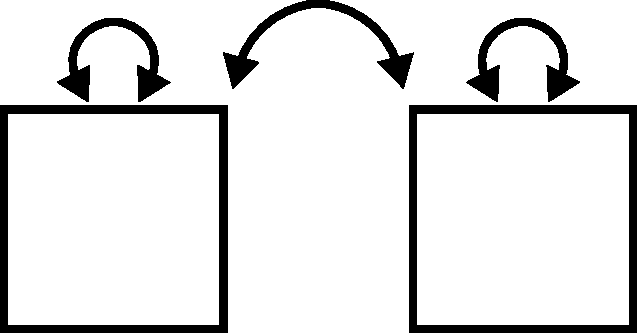
\includegraphics{graphics/covariance} \end{center}

\hypertarget{covariance-calculating}{%
\section{Calculating covariance}\label{covariance-calculating}}

The last chapter was about variance, which measures the spread of a single variable. Now we extend this idea to pairs of variables.

We say that two variables ``co-vary'' when the spread of one variable is related to the spread of another variable. This relationship represents an \emph{association} between the two variables.

We'll call our two variables \(X_{1}\) and \(X_{2}\). To keep things simple, let's assume that we have already mean centered our variables.

If \(X_{1}\) and \(X_{2}\) are already mean centered, then what are \(\overline{X_{1}}\) and \(\overline{X_{2}}\)?

As we did in the last chapter with variance, we'll build up the calculation of covariance step-by-step using a table to keep track of intermediate quantities we need.

Here are two variables (with \(n = 7\)) that have been mean centered:

\begin{longtable}[]{@{}rr@{}}
\toprule
\(X_{1}\) & \(X_{2}\) \\
\midrule
\endhead
-1 & -2 \\
-2 & 2 \\
2 & -2 \\
-3 & -1 \\
4 & 2 \\
-1 & -2 \\
1 & 3 \\
\bottomrule
\end{longtable}

Check that the mean of both columns is truly zero.

Something interesting happens when we look at the product \(X_{1}X_{2}\).

If \(X_{1}\) and \(X_{2}\) both lie above their means, they are both positive numbers. Therefore, their product is positive.

What if both \(X_{1}\) and \(X_{2}\) lie below their means? What do we know about their values individually and what do we know about their product?

Here is the chart again, but with the products listed in a new column:

\begin{longtable}[]{@{}rrr@{}}
\toprule
\(X_{1}\) & \(X_{2}\) & \(X_{1}X_{2}\) \\
\midrule
\endhead
-1 & -2 & 2 \\
-2 & 2 & -4 \\
2 & -2 & -4 \\
-3 & -1 & 3 \\
4 & 2 & 8 \\
-1 & -2 & 2 \\
1 & 3 & 3 \\
\bottomrule
\end{longtable}

Now we add up the products across all seven data pairs:

\begin{longtable}[]{@{}rrr@{}}
\toprule
\(X_{1}\) & \(X_{2}\) & \(X_{1}X_{2}\) \\
\midrule
\endhead
-1 & -2 & 2 \\
-2 & 2 & -4 \\
2 & -2 & -4 \\
-3 & -1 & 3 \\
4 & 2 & 8 \\
-1 & -2 & 2 \\
1 & 3 & 3 \\
& & Sum: 10 \\
\bottomrule
\end{longtable}

So when \(X_{1}\) and \(X_{2}\) tend to have similar values (both positive or both negative), their product is usually positive. It's not true of every pair of values in the table above; some products are negative. But the majority are positive. Therefore, the sum of all such products will be positive.

We're almost there. Just like we wanted the average squared deviation to calculate the variance, here we want the average of the products from the third column above. And just like in the case of variance, it's not \emph{quite} the average we calculate. Instead of dividing by \(n\), we divide by \(n - 1\) for exactly the same esoteric reason. In our example, there are 7 data points (in other words, 7 rows of data), so we divide by 6.

Putting this all together:

\begin{longtable}[]{@{}rrr@{}}
\toprule
\(X_{1}\) & \(X_{2}\) & \(X_{1}X_{2}\) \\
\midrule
\endhead
-1 & -2 & 2 \\
-2 & 2 & -4 \\
2 & -2 & -4 \\
-3 & -1 & 3 \\
4 & 2 & 8 \\
-1 & -2 & 2 \\
1 & 3 & 3 \\
& & Sum: 10 \\
& & Covariance: 10/6 = \(\boxed{1.67}\) \\
\bottomrule
\end{longtable}

In our diagrams, the covariance of two variables is indicated by a curved, double-headed arrow pointing at both boxes and labeled with the value of the covariance, like this:

\begin{center}\includegraphics{graphics/covariance_labeled} \end{center}

Note that we still include the variances of each of the individual variables. They are still important to us. We just have one new type of arrow now.

Verify that the variances in the diagram are correct for our example. You can do it by hand if you want, but using R is fine too.

Here is the final formula for covariance, written as \(Cov\left(X_{1}, X_{2}\right)\). This works for all pairs of variables, even if they aren't mean centered. The terms \(\left(X_{1} - \overline{X_1}\right)\) and \(\left(X_{2} - \overline{X_2}\right)\) do the mean centering:

\[
Cov\left(X_{1}, X_{2}\right) = \frac{\sum \left(X_{1} - \overline{X_{1}}\right)\left(X_{2} - \overline{X_{2}}\right)}{n - 1}
\]

Suppose \(X_{1}\) tends to be above its mean when \(X_{2}\) is below its mean and \(X_{1}\) tends to be below its mean when \(X_{2}\) is above its mean. What will the product \(\left(X_{1} - \overline{X_{1}}\right)\left(X_{2} - \overline{X_{2}}\right)\) usually be? Therefore, what will the sum of all such products likely be?

For general variables (not necessarily mean centered), the table will actually look like this:

\begin{longtable}[]{@{}
  >{\raggedleft\arraybackslash}p{(\columnwidth - 8\tabcolsep) * \real{0.2000}}
  >{\raggedleft\arraybackslash}p{(\columnwidth - 8\tabcolsep) * \real{0.2000}}
  >{\raggedleft\arraybackslash}p{(\columnwidth - 8\tabcolsep) * \real{0.2000}}
  >{\raggedleft\arraybackslash}p{(\columnwidth - 8\tabcolsep) * \real{0.2000}}
  >{\raggedleft\arraybackslash}p{(\columnwidth - 8\tabcolsep) * \real{0.2000}}@{}}
\toprule
\begin{minipage}[b]{\linewidth}\raggedleft
\(X_{1}\)
\end{minipage} & \begin{minipage}[b]{\linewidth}\raggedleft
\(X_{2}\)
\end{minipage} & \begin{minipage}[b]{\linewidth}\raggedleft
\(\left(X_{1} - \overline{X_{1}}\right)\)
\end{minipage} & \begin{minipage}[b]{\linewidth}\raggedleft
\(\left(X_{2} - \overline{X_{2}}\right)\)
\end{minipage} & \begin{minipage}[b]{\linewidth}\raggedleft
\(\left(X_{1} - \overline{X_{1}}\right)\left(X_{2} - \overline{X_{2}}\right)\)
\end{minipage} \\
\midrule
\endhead
17 & 23 & -2 & 11 & -22 \\
25 & 15 & 6 & 3 & 18 \\
\ldots{} & \ldots{} & \ldots{} & \ldots{} & \ldots{} \\
\bottomrule
\end{longtable}

Calculate the covariance by hand by making a table like the one above. (These variables are \emph{not} mean centered, so you'll have to calculate the mean of each variable in order to fill out the third and fourth columns.)

\(X_{3}\): 8, 10, 16, 7, 4, 3

\(X_{4}\): 6, 5, 4, 9, 11, 7

Explain intuitively why the covariance is negative for these two variables.

When calculating variance, the order of the data points does not matter. Why?

When calculating covariance, the order of the data points \emph{does} matter. Why?

What if you keep pairs together, but rearrange the rows of the table. How does that affect the covariance?

\hypertarget{covariance-r}{%
\section{Calculating covariance in R}\label{covariance-r}}

Once we've done it by hand a few times to make sure we understand how the formula works, from here on out we can let R do the work for us:

\begin{Shaded}
\begin{Highlighting}[]
\NormalTok{X1 }\OtherTok{\textless{}{-}} \FunctionTok{c}\NormalTok{(}\SpecialCharTok{{-}}\DecValTok{1}\NormalTok{,}\SpecialCharTok{{-}}\DecValTok{2}\NormalTok{, }\DecValTok{2}\NormalTok{, }\SpecialCharTok{{-}}\DecValTok{3}\NormalTok{, }\DecValTok{4}\NormalTok{, }\SpecialCharTok{{-}}\DecValTok{1}\NormalTok{, }\DecValTok{1}\NormalTok{)}
\NormalTok{X2 }\OtherTok{\textless{}{-}} \FunctionTok{c}\NormalTok{(}\SpecialCharTok{{-}}\DecValTok{2}\NormalTok{, }\DecValTok{2}\NormalTok{, }\SpecialCharTok{{-}}\DecValTok{2}\NormalTok{, }\SpecialCharTok{{-}}\DecValTok{1}\NormalTok{, }\DecValTok{2}\NormalTok{, }\SpecialCharTok{{-}}\DecValTok{2}\NormalTok{, }\DecValTok{3}\NormalTok{)}
\FunctionTok{cov}\NormalTok{(X1, X2)}
\end{Highlighting}
\end{Shaded}

\begin{verbatim}
## [1] 1.666667
\end{verbatim}

\begin{Shaded}
\begin{Highlighting}[]
\NormalTok{X3 }\OtherTok{\textless{}{-}} \FunctionTok{c}\NormalTok{(}\DecValTok{8}\NormalTok{, }\DecValTok{10}\NormalTok{, }\DecValTok{16}\NormalTok{, }\DecValTok{7}\NormalTok{, }\DecValTok{4}\NormalTok{, }\DecValTok{3}\NormalTok{)}
\NormalTok{X4 }\OtherTok{\textless{}{-}} \FunctionTok{c}\NormalTok{(}\DecValTok{6}\NormalTok{, }\DecValTok{5}\NormalTok{, }\DecValTok{4}\NormalTok{, }\DecValTok{9}\NormalTok{, }\DecValTok{11}\NormalTok{, }\DecValTok{7}\NormalTok{)}
\FunctionTok{cov}\NormalTok{(X3, X4)}
\end{Highlighting}
\end{Shaded}

\begin{verbatim}
## [1] -9.2
\end{verbatim}

And here's some real world data:

\begin{Shaded}
\begin{Highlighting}[]
\FunctionTok{cov}\NormalTok{(airquality}\SpecialCharTok{$}\NormalTok{Temp, airquality}\SpecialCharTok{$}\NormalTok{Wind)}
\end{Highlighting}
\end{Shaded}

\begin{verbatim}
## [1] -15.27214
\end{verbatim}

\hypertarget{covariance-rules}{%
\section{Covariance rules}\label{covariance-rules}}

We'll think of the variance and covariance rules as one big list. We left off on \href{./variance.html\#Rule4}{\textbf{Rule 4}}, so now we'll introduce \protect\hyperlink{Rule5}{\textbf{Rule 5}}.

\begin{itemize}
\tightlist
\item
  \textbf{Rule 5}
\end{itemize}

\[
Cov(X, X) = Var(X)
\]

In words, \protect\hyperlink{Rule5}{\textbf{Rule 5}} states that the covariance of a variable \emph{with itself} is just the same thing as the variance of that variable. This is quite remarkable! It means that variance is really just a special case of covariance.

Explain why \protect\hyperlink{Rule5}{\textbf{Rule 5}} is true. (Hint: think about how you would calculate \(Cov(X, X)\) using either the formula or the table---or both!)

\begin{itemize}
\tightlist
\item
  \textbf{Rule 6}
\end{itemize}

\[
Cov\left(X_{1}, X_{2}\right) = Cov\left(X_{2}, X_{1}\right)
\]

In words, we would say that covariance is \emph{symmetric}.

Explain why \protect\hyperlink{Rule6}{\textbf{Rule 6}} is true. (Again, think about the formula or the table---or both!)

The next four rules are analogous to similar rules for variance (\href{./variance.html\#Rule1}{\textbf{Rule 1}}, \href{./variance.html\#Rule2}{\textbf{Rule 2}}, \href{./variance.html\#Rule3}{\textbf{Rule 3}}, and \href{./variance.html\#Rule4}{\textbf{Rule 4}}).

\begin{itemize}
\tightlist
\item
  \textbf{Rule 7}
\end{itemize}

Suppose that \(C\) is a ``constant'' variable, meaning that it always has the same value (rather than being a variable that could contain lots of different numbers). Then,

\[
Cov\left(X, C\right) = 0
\]

As always, try to explain this rule. Give an intuitive explanation of why this rule ``should'' be true. Then think about it computationally, thinking of either the formula or the table---or both!

\begin{itemize}
\tightlist
\item
  \textbf{Rule 8}
\end{itemize}

\[
Cov\left(X_{1} + X_{2}, X_{3}\right) = Cov\left(X_{1}, X_{3}\right) + Cov\left(X_{2}, X_{3}\right)  
\]

What you should appreciate here is that there is no longer any restriction on the relationships among the variables involved. \href{./variance.html\#Rule2}{\textbf{Rule 2}} only worked when the two variables were independent. On the other hand, \protect\hyperlink{Rule8}{\textbf{Rule 8}} works for any combination of variables, no matter their relation.

Even more satisfying is this next rule:

\begin{itemize}
\tightlist
\item
  \textbf{Rule 9}
\end{itemize}

\[
Cov\left(X_{1} - X_{2}, X_{3}\right) = Cov\left(X_{1}, X_{3}\right) - Cov\left(X_{2}, X_{3}\right)  
\]

Yay! The minus sign behaves sensibly now! Of course, since covariances can be positive or negative (unlike variances which are always positive!) we can more safely subtract two of them without worry. And this rule, like \protect\hyperlink{Rule8}{\textbf{Rule 8}}, does not depend on \(X_{1}\) and \(X_{2}\) being independent. They can be any two variables.

There are versions of these rules with the addition or subtraction on the other side, but these are just minor variations of \protect\hyperlink{Rule8}{\textbf{Rule 8}} and \protect\hyperlink{Rule9}{\textbf{Rule 9}}, so they're not worth mentioning as a separate rule. Remember that covariance is symmetric, so you can always swap things on the left and right of the comma.

\[
Cov\left(X_{1}, X_{2} \pm X_{3}\right) = Cov\left(X_{1}, X_{2}\right) \pm Cov\left(X_{1}, X_{3}\right)  
\]

\begin{itemize}
\tightlist
\item
  \textbf{Rule 10}
\end{itemize}

If \(a\) is any number,

\[
Cov\left(a X_{1}, X_{2}\right) = a Cov\left(X_{1}, X_{2}\right) =  Cov\left(X_{1}, a X_{2}\right)  
\]

This rule is also very sensible. Instead of \href{./variance.html\#Rule4}{\textbf{Rule 4}} that takes a number \(a\) and pulls out an \(a^{2}\), \protect\hyperlink{Rule10}{\textbf{Rule 10}} just pulls out a single factor of \(a\) (from either slot).

Just a couple more rules. We were talking about independence in conjunction with \protect\hyperlink{Rule8}{\textbf{Rule 8}} and \protect\hyperlink{Rule9}{\textbf{Rule 9}}. That leads directly to an interesting and super-important rule:

\begin{itemize}
\tightlist
\item
  \textbf{Rule 11}
\end{itemize}

If \(X_{1}\) and \(X_{2}\) are independent, then

\[
Cov\left(X_{1}, X_{2}\right) = 0
\]

Why is \protect\hyperlink{Rule11}{\textbf{Rule 11}} true, intuitively?

It's interesting to note that this rule only works one way. In other words, if you know that two variables are independent, then you can conclude their covariance is zero. However, if you know the covariance is zero, that doesn't necessarily mean that the two variables are independent. We'll see an example of this later in the chapter.

Finally, one rule to rule them all:

\begin{itemize}
\tightlist
\item
  \textbf{Rule 12}
\end{itemize}

For \emph{any} two variables \(X_{1}\) and \(X_{2}\):

\[
Var(aX_{1} + bX_{2}) = 
    a^2Var(X_{1}) + b^2Var(X_{2}) + 2abCov(X_{1}, X_{2})
\]

This brings practically everything we know together into one rule!

Proving \protect\hyperlink{Rule12}{\textbf{Rule 12}} will give us good practice with the type of manipulation we'll need to do in future chapters. So here goes. For the first few steps, you name what rule we're invoking. Then, you'll pick up the thread and follow it through the last few steps on your own.

\begin{align}
Var(aX_{1} + bX_{2}) &= Cov(aX_{1} + bX_{2}, aX_{1} + bX_{2}) \\
    &= Cov(aX_{1} + bX_{2}, aX_{1}) + Cov(aX_{1} + bX_{2}, bX_{2}) \\
    &=  Cov(aX_{1}, aX_{1}) + 
        Cov(bX_{2}, aX_{1}) + \\
    &   \qquad Cov(aX_{1}, bX_{2}) + 
        Cov(bX_{2}, bX_{2}) \\
    &= \quad ???
\end{align}

You'll need these rules to do calculations in future chapters. Rather than having to search for them in Chapter \ref{variance} and this chapter, we've gathered up all the rules in one convenient place in Appendix \ref{appendix-rules}.

\hypertarget{covariance-correlation}{%
\section{Correlation}\label{covariance-correlation}}

The pros and cons for calculating covariance are similar to those for variance. The mathematics is much nicer for covariance, but we lose interpretability.

Let's suppose that \(X_{1}\) measures salary in dollars and \(X_{2}\) measures years of education. We would expect there to be some association between these variables, so we calculate the covariance. What is the unit of measurement of the resulting number?

The solution to the problem here is not as simple as it was for variance. Since variance had squared units, all we had to do was take the square root. Covariance has a weird product of units, so we have to do something more clever.

Following up on the activity above, let's suppose we have a covariance with units of ``dollar-years''. If we divide by a number expressed in dollars, we get rid of those units and we're left with years. But that seems unsatisfying; covariance should express something about both variables that went into it. Likewise, it makes no sense to divide by a number expressed in years as that would leave us just with dollars.

The solution to the dilemma is to accept that we aren't going to be able to keep any units in a meaningful way. Therefore, what we want is something \emph{standardized}, meaning that it has no units.

If \(X_{1}\) is expressed in dollars, can you think of a statistic that measures spread and is also in units of dollars?

Likewise, if \(X_{2}\) is measured in years, what statistic that measures spread is also in units of years?

The previous activity gives us an idea. What if we divide the covariance by \emph{both} the standard deviation of \(X_{1}\) \emph{and} the standard deviation of \(X_{2}\)?

\[
\frac{Cov(X_{1},X_{2})}{SD(X_{1}) SD(X_{2})}
\]

Sometimes it's written like this:

\[
\frac{Cov(X_{1},X_{2})}{\sqrt{Var(X_{1})} \sqrt{Var(X_{2})}}
\]
But that's the same thing, right?

This quantity has no units. We call this the \emph{correlation} between \(X_{1}\) and \(X_{2}\). We'll either write
\[
Corr(X_{1}, X_{2})
\]
or, if we need to be more concise,
\[
r_{X_{1}X_{2}}
\]

Yes, this is the same as the correlation coefficient you learned about in your intro stats class, although it wasn't likely presented to you quite this way.\footnote{Karl Pearson is credited with inventing the correlation coefficient. Pearson was a life-long eugenicist and a proponent of using ``science'' to prove that some races were superior to others. It important to disentangle the truly valuable notion of correlation from the discredited hands that may have first written it down. Therefore, we will not be referring to it in this text as the Pearson correlation coefficient.}

One great thing about correlation is that it has no units, so it serves as a sort of ``universal'' measure of how two variables co-vary. But the best part is that it has a nice intuitive meaning precisely because it factors out the pieces of the covariance that are only there because of the spread of the two variables individually. In other words, the fact that \(X_{1}\) and \(X_{2}\) have their own variability actually \emph{complicates} the notion of covariance. Those individual variances ``corrupt'' the interpretation of covariance. But after excising them, all that's left in the correlation is the ``pure'' part of the covariance that expresses the relationship or association between \(X_{1}\) and \(X_{2}\).

\hypertarget{covariance-standardized}{%
\section{Covariance with standardized data}\label{covariance-standardized}}

In the last chapter, you showed that the variance of a standardized variable was 1. What is the covariance between two standardized variables?

Let's standardize both \(X_{1}\) and \(X_{2}\). To make the math a little easier, we'll use similar notation to what we used at the end of the last chapter.

\(M_{1} = \overline{X_{1}}\)

\(S_{1} = SD(X_{1})\)

\(M_{2} = \overline{X_{2}}\)

\(S_{2} = SD(X_{2})\)

And we'll write the z-scores in a way that is more amenable to mathematical manipulation (like before):

\[
Z_{1} = \frac{1}{S_{1}}\left(X_{1} - M_{1}\right)
\]

\[
Z_{2} = \frac{1}{S_{2}}\left(X_{2} - M_{2}\right)
\]

This looks a little more intimidating, but if you apply the rules, it works out:

\begin{align}
Cov(Z_{1}, Z_{2}) &= Cov\left( \frac{1}{S_{1}}\left(X_{1} - M_{1}\right), \frac{1}{S_{2}}\left(X_{2} - M_{2}\right) \right) \\
    &= \quad ???
\end{align}

Work this out. Take your time. Apply the rules carefully. So that you know what you're aiming for, you should get

\[
Cov(Z_{1}, Z_{2}) = \frac{Cov\left( X_{1}, X_{2} \right)}{S_{1} S_{2}}
\]

Okay, now remember that \(S_{1}\) is just a convenient substitute for \(SD(X_{1})\) and \(S_{2}\) is just a substitute for \(SD(X_{2})\). Wait, does that answer look familiar?

This is cool! Correlation is simply the covariance of two variables after they've been standardized.

This also reinforces the earlier comment about interpreting covariance after removing the extraneous influence of the spread of the individual variables. Standardizing variables makes the spread all all variables 1, so their covariance is now a pure representation of just the association between them.

You probably remember from intro stats that correlation takes on values between -1 and 1. That fact is not obvious from the formula we have. Why should the fraction
\[
\frac{Cov(X_{1},X_{2})}{SD(X_{1}) SD(X_{2})}
\]
be bounded by -1 and 1?

Let's go back to standardized variable to keep things simple. The correlation is just the covariance of two standardized variables:

\[
Corr(X_{1}, X_{2}) = Cov(Z_{1}, Z_{2})
\]

Use the rules to calculate this:

\[
Var(Z_{1} + Z_{2})
\]

Remember that \(Z_{1}\) and \(Z_{2}\) are not necessarily independent. (In fact, we hope they are not. Otherwise, why do we care about their correlation? It would be zero!) So you need \protect\hyperlink{Rule12}{\textbf{Rule 12}}, not \href{./variance.html\#Rule2}{\textbf{Rule 2}}. Keep manipulating until you get
\[
2 + 2Corr(X_{1}, X_{2})
\]

Since variances are always non-negative, we now know that

\[
0 \leq 2 + 2Corr(X_{1}, X_{2})
\]
Solve this inequality for \(Corr(X_{1}, X_{2})\).

Now follow the exact same steps for
\[
Var(Z_{1} - Z_{2})
\]

Very little should change in your answer, but there is one small change. Again, solve the resulting inequality. (Don't forget the key rule when working with inequalities that multiplying or dividing by a negative number changes the direction of the inequality.)

Here is a fact we will state without proof:

Correlation is only interpretable as the strength of \textbf{linear} associations.

Why is this? Basically, it boils down to the fact that a ``perfect'' correlation of 1 or -1 is only achievable when data points lie on a perfectly straight line. Therefore, thinking of correlation as lying between 0 and 1 (or 0 and -1) is only sensible if you are judging how close points are to lying on a straight line. We'll see examples of this in the next section when we plot some data.

To calculation correlation in R, use the \texttt{cor} command:

\begin{Shaded}
\begin{Highlighting}[]
\FunctionTok{cor}\NormalTok{(airquality}\SpecialCharTok{$}\NormalTok{Temp, airquality}\SpecialCharTok{$}\NormalTok{Wind)}
\end{Highlighting}
\end{Shaded}

\begin{verbatim}
## [1] -0.4579879
\end{verbatim}

Use R to confirm that the number above is the covariance divided by the product of the standard deviations.

\hypertarget{covariance-visualizing}{%
\section{Visualizing correlation}\label{covariance-visualizing}}

Covariance is hard to interpret, so when we're visualizing data and we want to understand any association that might exist between two variables, correlation is a much better statistic to calculate. Let's see how correlation relates to the graph of two variables.

Before getting into the graphing, we will need to load some packages. The \texttt{tidyverse} is a whole set of commonly used packages that will allow us to work with data frames (or ``tibbles'' as the cool kids are calling them) and make graphs. Be sure to load the package by typing the following in R before going any further:

\begin{Shaded}
\begin{Highlighting}[]
\FunctionTok{library}\NormalTok{(tidyverse)}
\end{Highlighting}
\end{Shaded}

\begin{verbatim}
## -- Attaching packages --------------------------------------- tidyverse 1.3.1 --
\end{verbatim}

\begin{verbatim}
## v ggplot2 3.3.6     v purrr   0.3.4
## v tibble  3.1.7     v dplyr   1.0.9
## v tidyr   1.2.0     v stringr 1.4.0
## v readr   2.1.2     v forcats 0.5.1
\end{verbatim}

\begin{verbatim}
## -- Conflicts ------------------------------------------ tidyverse_conflicts() --
## x dplyr::filter() masks stats::filter()
## x dplyr::lag()    masks stats::lag()
\end{verbatim}

In fact, from here on out, we'll start each chapter by loading any necessary libraries in R that we'll need.

The standard graph of two numerical variables is a scatterplot. Let's start with a straight line relationship. First, we define two variables. We'll use some shortcuts here to make our lives a little easier. The \texttt{seq} command just generates a sequence of numbers.

\begin{Shaded}
\begin{Highlighting}[]
\NormalTok{X5 }\OtherTok{\textless{}{-}} \FunctionTok{seq}\NormalTok{(}\DecValTok{1}\NormalTok{, }\DecValTok{9}\NormalTok{)}
\NormalTok{X5}
\end{Highlighting}
\end{Shaded}

\begin{verbatim}
## [1] 1 2 3 4 5 6 7 8 9
\end{verbatim}

Then we can establish a linear relationship just by declaring one in a formula:

\begin{Shaded}
\begin{Highlighting}[]
\NormalTok{X6 }\OtherTok{\textless{}{-}} \DecValTok{3} \SpecialCharTok{+} \FloatTok{0.5} \SpecialCharTok{*}\NormalTok{ X5}
\NormalTok{X6}
\end{Highlighting}
\end{Shaded}

\begin{verbatim}
## [1] 3.5 4.0 4.5 5.0 5.5 6.0 6.5 7.0 7.5
\end{verbatim}

To put both variables into the same graph, it helps to make them both columns in a single tibble.

\begin{Shaded}
\begin{Highlighting}[]
\NormalTok{linear\_data }\OtherTok{\textless{}{-}} \FunctionTok{tibble}\NormalTok{(X5, X6)}
\NormalTok{linear\_data}
\end{Highlighting}
\end{Shaded}

\begin{verbatim}
## # A tibble: 9 x 2
##      X5    X6
##   <int> <dbl>
## 1     1   3.5
## 2     2   4  
## 3     3   4.5
## 4     4   5  
## 5     5   5.5
## 6     6   6  
## 7     7   6.5
## 8     8   7  
## 9     9   7.5
\end{verbatim}

And here is the graph:

\begin{Shaded}
\begin{Highlighting}[]
\FunctionTok{ggplot}\NormalTok{(linear\_data, }\FunctionTok{aes}\NormalTok{(}\AttributeTok{y =}\NormalTok{ X6, }\AttributeTok{x =}\NormalTok{ X5)) }\SpecialCharTok{+}
    \FunctionTok{geom\_point}\NormalTok{()}
\end{Highlighting}
\end{Shaded}

\includegraphics{sem_book_files/figure-latex/unnamed-chunk-34-1.pdf}

Now the correlation:

\begin{Shaded}
\begin{Highlighting}[]
\FunctionTok{cor}\NormalTok{(X5, X6)}
\end{Highlighting}
\end{Shaded}

\begin{verbatim}
## [1] 1
\end{verbatim}

It is 1, as expected.

What about a perfectly straight line with a negative slope?

\begin{Shaded}
\begin{Highlighting}[]
\NormalTok{X7 }\OtherTok{\textless{}{-}} \DecValTok{5} \SpecialCharTok{{-}} \FloatTok{0.2} \SpecialCharTok{*}\NormalTok{ X5}
\NormalTok{X7}
\end{Highlighting}
\end{Shaded}

\begin{verbatim}
## [1] 4.8 4.6 4.4 4.2 4.0 3.8 3.6 3.4 3.2
\end{verbatim}

Throw this new variable into the tibble we already have (for convenience). To explain the syntax below, the \texttt{\%\textgreater{}\%} symbol is called a ``pipe'' and it tells R to pass the \texttt{linear\_data} tibble on to the next row to process it. And the processing itself is dictated by the \texttt{bind\_cols} command which tells R to ``bind a new column'' to the tibble. The part that says \texttt{X7\ =\ X7} may be a little confusing. It says to add the new column \texttt{X7}, but also still call it \texttt{X7}.

\begin{Shaded}
\begin{Highlighting}[]
\NormalTok{linear\_data }\OtherTok{\textless{}{-}}\NormalTok{ linear\_data }\SpecialCharTok{\%\textgreater{}\%}
    \FunctionTok{bind\_cols}\NormalTok{(}\AttributeTok{X7 =}\NormalTok{ X7)}
\NormalTok{linear\_data}
\end{Highlighting}
\end{Shaded}

\begin{verbatim}
## # A tibble: 9 x 3
##      X5    X6    X7
##   <int> <dbl> <dbl>
## 1     1   3.5   4.8
## 2     2   4     4.6
## 3     3   4.5   4.4
## 4     4   5     4.2
## 5     5   5.5   4  
## 6     6   6     3.8
## 7     7   6.5   3.6
## 8     8   7     3.4
## 9     9   7.5   3.2
\end{verbatim}

\begin{Shaded}
\begin{Highlighting}[]
\FunctionTok{ggplot}\NormalTok{(linear\_data, }\FunctionTok{aes}\NormalTok{(}\AttributeTok{y =}\NormalTok{ X7, }\AttributeTok{x =}\NormalTok{ X5)) }\SpecialCharTok{+}
    \FunctionTok{geom\_point}\NormalTok{()}
\end{Highlighting}
\end{Shaded}

\includegraphics{sem_book_files/figure-latex/unnamed-chunk-38-1.pdf}

\begin{Shaded}
\begin{Highlighting}[]
\FunctionTok{cor}\NormalTok{(X5, X7)}
\end{Highlighting}
\end{Shaded}

\begin{verbatim}
## [1] -1
\end{verbatim}

Again, that is what we expected.

What happens if we plot random data? The \texttt{runif} command just chooses random numbers uniformly between 0 and 1.\footnote{Sean's brain always want to parse this command as ``run if''. Run if what? No, no, it's ``r unif''.}

\begin{Shaded}
\begin{Highlighting}[]
\FunctionTok{set.seed}\NormalTok{(}\DecValTok{1234}\NormalTok{)}
\NormalTok{X8 }\OtherTok{\textless{}{-}} \FunctionTok{runif}\NormalTok{(}\DecValTok{20}\NormalTok{)}
\NormalTok{X9 }\OtherTok{\textless{}{-}} \FunctionTok{runif}\NormalTok{(}\DecValTok{20}\NormalTok{)}
\end{Highlighting}
\end{Shaded}

\begin{Shaded}
\begin{Highlighting}[]
\NormalTok{X8}
\end{Highlighting}
\end{Shaded}

\begin{verbatim}
##  [1] 0.113703411 0.622299405 0.609274733 0.623379442 0.860915384 0.640310605
##  [7] 0.009495756 0.232550506 0.666083758 0.514251141 0.693591292 0.544974836
## [13] 0.282733584 0.923433484 0.292315840 0.837295628 0.286223285 0.266820780
## [19] 0.186722790 0.232225911
\end{verbatim}

\begin{Shaded}
\begin{Highlighting}[]
\NormalTok{X9}
\end{Highlighting}
\end{Shaded}

\begin{verbatim}
##  [1] 0.31661245 0.30269337 0.15904600 0.03999592 0.21879954 0.81059855
##  [7] 0.52569755 0.91465817 0.83134505 0.04577026 0.45609148 0.26518667
## [13] 0.30467220 0.50730687 0.18109621 0.75967064 0.20124804 0.25880982
## [19] 0.99215042 0.80735234
\end{verbatim}

\begin{Shaded}
\begin{Highlighting}[]
\NormalTok{random\_data }\OtherTok{\textless{}{-}} \FunctionTok{tibble}\NormalTok{(X8, X9)}
\NormalTok{random\_data}
\end{Highlighting}
\end{Shaded}

\begin{verbatim}
## # A tibble: 20 x 2
##         X8     X9
##      <dbl>  <dbl>
##  1 0.114   0.317 
##  2 0.622   0.303 
##  3 0.609   0.159 
##  4 0.623   0.0400
##  5 0.861   0.219 
##  6 0.640   0.811 
##  7 0.00950 0.526 
##  8 0.233   0.915 
##  9 0.666   0.831 
## 10 0.514   0.0458
## 11 0.694   0.456 
## 12 0.545   0.265 
## 13 0.283   0.305 
## 14 0.923   0.507 
## 15 0.292   0.181 
## 16 0.837   0.760 
## 17 0.286   0.201 
## 18 0.267   0.259 
## 19 0.187   0.992 
## 20 0.232   0.807
\end{verbatim}

\begin{Shaded}
\begin{Highlighting}[]
\FunctionTok{ggplot}\NormalTok{(random\_data, }\FunctionTok{aes}\NormalTok{(}\AttributeTok{y =}\NormalTok{ X9, }\AttributeTok{x =}\NormalTok{ X8)) }\SpecialCharTok{+}
    \FunctionTok{geom\_point}\NormalTok{()}
\end{Highlighting}
\end{Shaded}

\includegraphics{sem_book_files/figure-latex/unnamed-chunk-44-1.pdf}

What do you guess is the correlation between \(X_{8}\) and \(X_{9}\)?

Now calculate it using R? Did you get the \emph{exact} answer you guessed? If not, why not?

What about data that follows a perfect mathematical relationship that is not a straight line? For example, here is a part of a parabola.

\begin{Shaded}
\begin{Highlighting}[]
\NormalTok{X10 }\OtherTok{\textless{}{-}} \FloatTok{0.1} \SpecialCharTok{*}\NormalTok{ X5}\SpecialCharTok{\^{}}\DecValTok{2}
\NormalTok{X10}
\end{Highlighting}
\end{Shaded}

\begin{verbatim}
## [1] 0.1 0.4 0.9 1.6 2.5 3.6 4.9 6.4 8.1
\end{verbatim}

\begin{Shaded}
\begin{Highlighting}[]
\NormalTok{nonlinear\_data }\OtherTok{\textless{}{-}} \FunctionTok{tibble}\NormalTok{(X5, X10)}
\NormalTok{nonlinear\_data}
\end{Highlighting}
\end{Shaded}

\begin{verbatim}
## # A tibble: 9 x 2
##      X5   X10
##   <int> <dbl>
## 1     1   0.1
## 2     2   0.4
## 3     3   0.9
## 4     4   1.6
## 5     5   2.5
## 6     6   3.6
## 7     7   4.9
## 8     8   6.4
## 9     9   8.1
\end{verbatim}

\begin{Shaded}
\begin{Highlighting}[]
\FunctionTok{ggplot}\NormalTok{(nonlinear\_data, }\FunctionTok{aes}\NormalTok{(}\AttributeTok{y =}\NormalTok{ X10, }\AttributeTok{x =}\NormalTok{ X5)) }\SpecialCharTok{+}
    \FunctionTok{geom\_point}\NormalTok{()}
\end{Highlighting}
\end{Shaded}

\includegraphics{sem_book_files/figure-latex/unnamed-chunk-47-1.pdf}

Now for the correlation:

\begin{Shaded}
\begin{Highlighting}[]
\FunctionTok{cor}\NormalTok{(X5, X10)}
\end{Highlighting}
\end{Shaded}

\begin{verbatim}
## [1] 0.975281
\end{verbatim}

This is a large correlation, but it is not exactly 1, even though the points follow a precise mathematical relationship. That relationship is not linear.

Here's a fascinating example. For this, we'll want a parabola that goes down and then up.

\begin{Shaded}
\begin{Highlighting}[]
\NormalTok{X11 }\OtherTok{\textless{}{-}} \FloatTok{0.5} \SpecialCharTok{*}\NormalTok{ (X5 }\SpecialCharTok{{-}} \DecValTok{5}\NormalTok{)}\SpecialCharTok{\^{}}\DecValTok{2}
\NormalTok{X11}
\end{Highlighting}
\end{Shaded}

\begin{verbatim}
## [1] 8.0 4.5 2.0 0.5 0.0 0.5 2.0 4.5 8.0
\end{verbatim}

\begin{Shaded}
\begin{Highlighting}[]
\NormalTok{nonlinear\_data }\OtherTok{\textless{}{-}}\NormalTok{ nonlinear\_data }\SpecialCharTok{\%\textgreater{}\%}
    \FunctionTok{bind\_cols}\NormalTok{(}\AttributeTok{X11 =}\NormalTok{ X11)}
\NormalTok{nonlinear\_data}
\end{Highlighting}
\end{Shaded}

\begin{verbatim}
## # A tibble: 9 x 3
##      X5   X10   X11
##   <int> <dbl> <dbl>
## 1     1   0.1   8  
## 2     2   0.4   4.5
## 3     3   0.9   2  
## 4     4   1.6   0.5
## 5     5   2.5   0  
## 6     6   3.6   0.5
## 7     7   4.9   2  
## 8     8   6.4   4.5
## 9     9   8.1   8
\end{verbatim}

\begin{Shaded}
\begin{Highlighting}[]
\FunctionTok{ggplot}\NormalTok{(nonlinear\_data, }\FunctionTok{aes}\NormalTok{(}\AttributeTok{y =}\NormalTok{ X11, }\AttributeTok{x =}\NormalTok{ X5)) }\SpecialCharTok{+}
    \FunctionTok{geom\_point}\NormalTok{()}
\end{Highlighting}
\end{Shaded}

\includegraphics{sem_book_files/figure-latex/unnamed-chunk-51-1.pdf}

Before looking at the answer, what is your guess for the correlation between \(X_{5}\) and \(X_{11}\)?

Now calculate the correlation in R.

Again, there's a perfect mathematical relationship between these two variables. They are most definitely associated. So why is the correlation 0?

Recall the earlier promise to discuss \protect\hyperlink{Rule11}{\textbf{Rule 11}}. If two variables are independent, then their covariance is zero, and, therefore, their correlation is also zero. However, this rule doesn't work the other way around. The claim is that knowing the covariance/correlation is zero does not imply (necessarily) that the two variables are independent. Here is the promised example of that phenomenon. \(X_{5}\) and \(X_{11}\) have zero correlation. And yet, \(X_{5}\) and \(X_{11}\) are definitely \emph{not} independent.

This is important enough for a fancy box:

\textbf{When you see that the correlation between two variables is zero or near zero, be careful not to conclude that the variables are independent.}

A zero or near-zero correlation indicates only the lack of a \emph{linear} association between two variables. There may be nonlinear associations. That's why it's always a good idea to graph your data.

Real data is, of course, much messier and it's just not possible to have perfect correlations between two variables measured out there in the real world. (If you do find a perfect correlation between two columns of your data, chances are that you either recorded the same column twice, or the second column is some simple transformation of first column, like multiplying every value by the same number or something like that.)

Here is a plot of the temperature (degrees Fahrenheit) and wind speed (mph) from the New York air quality data set.

\begin{Shaded}
\begin{Highlighting}[]
\FunctionTok{ggplot}\NormalTok{(airquality, }\FunctionTok{aes}\NormalTok{(}\AttributeTok{y =}\NormalTok{ Temp, }\AttributeTok{x =}\NormalTok{ Wind)) }\SpecialCharTok{+}
    \FunctionTok{geom\_point}\NormalTok{()}
\end{Highlighting}
\end{Shaded}

\includegraphics{sem_book_files/figure-latex/unnamed-chunk-52-1.pdf}

Just looking at the scatterplot (without calculating anything), is the correlation between these two variables positive or negative? Try guessing the exact value of the correlation.

Now calculate the exact value of the correlation to see how close you were.

If you want some practice with looking at scatterplots and guessing the correlation, try this online game:

\href{http://guessthecorrelation.com/}{Guess the Correlation}

Turn up the sound! If the whole class plays at the same time, your classroom will sound like an arcade. Compete with your classmates to see who can get the high score.

\hypertarget{simple}{%
\chapter{Simple regression}\label{simple}}

\begin{center}\includegraphics{graphics/simple_regression} \end{center}

\hypertarget{preliminaries}{%
\section*{Preliminaries}\label{preliminaries}}
\addcontentsline{toc}{section}{Preliminaries}

We need to load the packages we will need for this chapter. The \texttt{tidyverse} package has all sorts of utilities for working with tibbles (data frames). The \texttt{broom} package will be used to calculate and store the residuals of the model. This will also be our first introduction to the \texttt{lavaan} package that will be used throughout the rest of the book.

\begin{Shaded}
\begin{Highlighting}[]
\FunctionTok{library}\NormalTok{(tidyverse)}
\FunctionTok{library}\NormalTok{(broom)}
\FunctionTok{library}\NormalTok{(lavaan)}
\end{Highlighting}
\end{Shaded}

\begin{verbatim}
## This is lavaan 0.6-11
## lavaan is FREE software! Please report any bugs.
\end{verbatim}

\hypertarget{simple-prediction}{%
\section{Prediction}\label{simple-prediction}}

One of the most important tasks in statistics is \emph{prediction}. Given some data, can we predict the value of something important about a population of interest?

Suppose you have gathered some data on anxiety among Utah high school students. There are various instruments available for measuring anxiety, so say you have administered the \href{https://en.wikipedia.org/wiki/Beck_Anxiety_Inventory}{Beck Anxiety Inventory}. This instrument assigns a score from 0 to 63, with lower numbers indicating less anxiety and higher numbers indicating more.

You take care to make sure your sample is as close to a simple random sample as possible so that it's representative of the population (all high school students in the state of Utah). From your sample data, you can calculate summary statistics. For example, you might find that the mean anxiety score for Utah high school students is 7.1 with a standard deviation of 3.9.

A random Utah high school student walks through the door. You don't know anything about them. Can you say anything about their anxiety? What is your best guess as to what their score might be on the Beck Anxiety Inventory?

We can do a lot better if we have another variable we can measure. For example, let's suppose our data records not only anxiety, but also the minutes of smart phone usage per day.

In theory, why would having information about smart phone usage potentially help us make better predictions of anxiety?

Do you suspect that the association between anxiety and smart phone usage is positive or negative? (You can Google this question to check if there is any empirical evidence out there for your guess.)

Now imagine that another random Utah high school student walks through the door. This time, I tell you that their smart phone usage is average (sitting at the mean). What is your best prediction for their anxiety score? (Give an exact value.)

What if I told you that the student who walked through the door had \emph{higher} than average smart phone usage? What would be your prediction of their anxiety score? (You can't give an exact value here, but give a qualitatively sensible answer.)

What if I told you that the student who walked through the door had \emph{lower} than average smart phone usage? What would be your prediction of their anxiety score? (Again, just give a qualitatively sensible answer.)

\hypertarget{simple-terminology}{%
\section{Regression terminology}\label{simple-terminology}}

When we have one variable we suspect may help us predict another variable, one way to study it is using a simple regression model.

This is related to, but somewhat different from, covariance. Covariance is symmetric, so it expresses the idea that two variables are mutually related. But there is no ``directionality'' to that relationship. By way of contrast, a simple regression model asserts that one of the variables is ``explanatory'' and the other is ``response''. In other words, we start with the values or properties of the explanatory variable and try to deduce what we can about the values or properties of the response variable.

Keep in mind that ``directionality'' is not the same as ``causality''. While it's possible that one variable causes another, there needs to be a data collection process (often a carefully controlled experiment) and a clear scientific rationale that justifies a causal relationship between variables before we can start thinking about inferring causality. For purposes of much of this book, directionality just means that we wish to establish a predictive relationship wherein we start with the properties of one variable and try to predict the properties of another variable. There is often a ``sensible'' order in which to do this based on the research questions asked or the hypotheses posed.

There are many different terminological conventions in statistics, so be aware that ``explanatory'' variables are also called---often depending on the discipline and the context---predictors, features, covariates, controls, regressors, inputs, or independent variables. In fact, in the context of structural equation modeling, we will use the term ``exogenous'' to refer to variables that play this role. (That term has a much more precise definition that we'll discuss in future chapters.) And ``response'' variables might be called outcomes, outputs, targets, explained variables, or dependent variables, among others. In this book, we will often use the term ``endogenous'' (again, in a very specific way yet to be explained). If there is a data collection process and a clear scientific rationale that justifies a causal relationship between variables, then we might be able to refer to variables as either ``cause'' or ``effect''.

Keep in mind that it's the scientific question we want to ask that determines the explanatory/response relationship. A different researcher with a different hypothesis might use the same two variables but with the roles reversed.

In the anxiety/smart-phone example above, which variable is explanatory and which is response, at least according to the way we stated the scenario?

\hypertarget{simple-model}{%
\section{The simple regression model}\label{simple-model}}

Here is the figure from the top of the chapter, only now we have decorated it with some letters (and a number):

\begin{center}\includegraphics{graphics/simple_regression_params} \end{center}

The goal of this section is to explain all these.

The variable names are \(X\) and \(Y\). \(X\) is the exogenous variable and \(Y\) is the endogenous variable. For example, \(X\) might be smart phone usage and \(Y\) might be the anxiety score from the example above. In this section, we're going to do some concrete calculations using the example from the last chapter about wind speed and temperature from the \texttt{airquality} data set. In the last chapter, we simply calculated the (symmetric) correlation between wind speed and temperature. Here, we will consider wind speed as exogenous and temperature as endogenous. In other words, our goal is to use the wind speed as a predictor of temperature.

The letter \(v\) requires no further explanation. This is the variance of the variable \(X\), so we already know about it.

The parameter \(b\) is supposed to measure something about the predictive relationship between \(X\) and \(Y\). It is attached to an arrow that is drawn a little thicker than the other arrows in the diagram. More to say about that in a moment.

The really weird, new part is the circle on the right. This will be the ``error'' term.

What is ``error'' and why is it here? To illustrate, let's plot wind speed against temperature. Before plotting and analyzing these variables, we are going to mean-center them and put them in a tibble.

\begin{Shaded}
\begin{Highlighting}[]
\NormalTok{X }\OtherTok{\textless{}{-}}\NormalTok{ airquality}\SpecialCharTok{$}\NormalTok{Wind }\SpecialCharTok{{-}} \FunctionTok{mean}\NormalTok{(airquality}\SpecialCharTok{$}\NormalTok{Wind)}
\NormalTok{Y }\OtherTok{\textless{}{-}}\NormalTok{ airquality}\SpecialCharTok{$}\NormalTok{Temp }\SpecialCharTok{{-}} \FunctionTok{mean}\NormalTok{(airquality}\SpecialCharTok{$}\NormalTok{Temp)}
\NormalTok{airquality\_mc }\OtherTok{\textless{}{-}} \FunctionTok{tibble}\NormalTok{(X, Y)}
\NormalTok{airquality\_mc}
\end{Highlighting}
\end{Shaded}

\begin{verbatim}
## # A tibble: 153 x 2
##        X      Y
##    <dbl>  <dbl>
##  1 -2.56 -10.9 
##  2 -1.96  -5.88
##  3  2.64  -3.88
##  4  1.54 -15.9 
##  5  4.34 -21.9 
##  6  4.94 -11.9 
##  7 -1.36 -12.9 
##  8  3.84 -18.9 
##  9 10.1  -16.9 
## 10 -1.36  -8.88
## # ... with 143 more rows
\end{verbatim}

\begin{Shaded}
\begin{Highlighting}[]
\FunctionTok{ggplot}\NormalTok{(airquality\_mc, }\FunctionTok{aes}\NormalTok{(}\AttributeTok{y =}\NormalTok{ Y, }\AttributeTok{x =}\NormalTok{ X)) }\SpecialCharTok{+}
    \FunctionTok{geom\_point}\NormalTok{()}
\end{Highlighting}
\end{Shaded}

\includegraphics{sem_book_files/figure-latex/unnamed-chunk-57-1.pdf}

Note that the exogenous variable (wind speed) is on the x-axis and the endogenous variable (temperature) is on the y-axis.

We can see a negative and reasonably linear association between these variables, so let's add a line of best fit to the data.

\begin{Shaded}
\begin{Highlighting}[]
\FunctionTok{ggplot}\NormalTok{(airquality\_mc, }\FunctionTok{aes}\NormalTok{(}\AttributeTok{y =}\NormalTok{ Y, }\AttributeTok{x =}\NormalTok{ X)) }\SpecialCharTok{+}
    \FunctionTok{geom\_point}\NormalTok{() }\SpecialCharTok{+}
    \FunctionTok{geom\_smooth}\NormalTok{(}\AttributeTok{method =}\NormalTok{ lm, }\AttributeTok{se =} \ConstantTok{FALSE}\NormalTok{)}
\end{Highlighting}
\end{Shaded}

\begin{verbatim}
## `geom_smooth()` using formula 'y ~ x'
\end{verbatim}

\includegraphics{sem_book_files/figure-latex/unnamed-chunk-58-1.pdf}

The line passes right through the origin \((0, 0)\). Why?

The slope of this line is \(-1.23\). We'll see how to calculate this slope in a bit. But what does this slope mean?

Look at the help file for the \texttt{airquality} data set. (Either use the Help tab in RStudio or type \texttt{?airquality} at the Console.)

What are the units of measurement of \(X\)? What are the units of measurement of \(Y\)? Since slope is ``rise over run'', what are the units of the slope?

So, the idea is that for every additional mile per hour of wind speed, we predict that the temperature goes down by 1.23 degrees Fahrenheit.

Why is the following sentence incorrect?

\begin{quote}
For every additional mile per hour of wind speed, the temperature goes down by 1.23 degrees Fahrenheit.
\end{quote}

The point is that the line is a \emph{model} that makes predictions. As long as \(X\) and \(Y\) are both mean-centered, the equation of this line is

\[
\hat{Y} = bX
\]

There is a new piece of notation here: \(\hat{Y}\). This symbol represents the \emph{predicted} value of \(Y\) according to the model. We will not get the \emph{actual} value of \(Y\) from this piece of the model because the actual values of \(Y\) differ from the model because real-world data doesn't lie on a perfect straight line. More on that in a moment.

According to the information above, we can estimate that the value of \(b\) is \(-1.23\):

\[
\hat{Y} = -1.23X
\]

This is a multiplicative effect. Again, as long as \(X\) and \(Y\) are both mean-centered, knowing the value of \(X\) allows us to predict the value of \(Y\) by multiplying by \(b\).

But those predictions will almost always be wrong. On any given day, given an increase of 1 mile per hour wind in wind speed, it will very rarely happen that the temperature will drop by \emph{exactly} 1.23 degrees. That's just a sort of ``average'' over time. On average, there's a slight temperature change associated with 1 mph change in wind speed, and the number -1.23 is the best estimate of that average change across our whole data set. We need to be \emph{especially} clear that an increase in wind speed does not necessary \emph{cause} a drop in temperature. I mean, that might be partially true, but we can't prove it from our observational data. There are all sorts of other reasons to explain both an increase in wind speed and a drop in temperature (like a cold front moving in).

Since our predictions are average effects and not specific guarantees, every prediction we make will be wrong by some amount. (We could get extremely lucky, but even then, it's difficult to imagine a situation in which our prediction is precisely correct to, say, 10 decimal places or something like that.) Therefore, there is error in our prediction. The new equation---accounting for error---is

\[
Y = bX + E
\]
or
\[
Y = -1.23X + E
\]

Now we use \(Y\) instead of \(\hat{Y}\). Once we include the error, we can recover the exact value of \(Y\), so this is no longer just a prediction from the straight-line model. Remember this:

If you write down a regression equation for an endogenous variable that includes all incoming arrows, \emph{including the residual error term}, use \(Y\).

If you write down a regression equation for an endogenous variable that includes all incoming arrows, \emph{excluding the residual error term}, use \(\hat{Y}\).

Error is a funny word because it has a negative connotation. It sounds like we made a mistake. Well, the model does make mistakes. Every model prediction is technically wrong. But this is not the kind of mistake that results from doing our arithmetic wrong or anything like that. It's simply the ``natural'' error that results from the messiness of the real world and the impossibility of predicting anything with certainty. For this reason, we will often prefer the term ``residual''. It's what is ``left over'' after we have made a prediction. It's the extra change in temperature, for example, that is not accounted for by the model with wind speed alone.

The residuals are evident in the plot above. If there were no residuals, every data point would lie on a perfect straight line. But the data points are all either a little above or below the line. Those vertical distances between the data and the line are the residuals or errors. Here is an example of two residuals plotted below in red.

\begin{Shaded}
\begin{Highlighting}[]
\FunctionTok{ggplot}\NormalTok{(airquality\_mc, }\FunctionTok{aes}\NormalTok{(}\AttributeTok{y =}\NormalTok{ Y, }\AttributeTok{x =}\NormalTok{ X)) }\SpecialCharTok{+}
    \FunctionTok{geom\_point}\NormalTok{() }\SpecialCharTok{+}
    \FunctionTok{geom\_smooth}\NormalTok{(}\AttributeTok{method =}\NormalTok{ lm, }\AttributeTok{se =} \ConstantTok{FALSE}\NormalTok{) }\SpecialCharTok{+}
    \FunctionTok{annotate}\NormalTok{(}\StringTok{"segment"}\NormalTok{,}
             \AttributeTok{x =} \SpecialCharTok{{-}}\FloatTok{2.56}\NormalTok{, }\AttributeTok{y =} \FloatTok{3.15}\NormalTok{,}
             \AttributeTok{xend =} \SpecialCharTok{{-}}\FloatTok{2.56}\NormalTok{, }\AttributeTok{yend =} \FloatTok{3.15} \SpecialCharTok{{-}} \FloatTok{14.03}\NormalTok{,}
             \AttributeTok{color =} \StringTok{"red"}\NormalTok{, }\AttributeTok{size =} \FloatTok{1.5}\NormalTok{) }\SpecialCharTok{+}
    \FunctionTok{annotate}\NormalTok{(}\StringTok{"segment"}\NormalTok{,}
             \AttributeTok{x =} \FloatTok{4.94}\NormalTok{, }\AttributeTok{y =} \SpecialCharTok{{-}}\FloatTok{6.08}\NormalTok{,}
             \AttributeTok{xend =} \FloatTok{4.94}\NormalTok{, }\AttributeTok{yend =} \SpecialCharTok{{-}}\FloatTok{6.08} \SpecialCharTok{+} \FloatTok{9.20}\NormalTok{,}
             \AttributeTok{color =} \StringTok{"red"}\NormalTok{, }\AttributeTok{size =} \FloatTok{1.5}\NormalTok{)}
\end{Highlighting}
\end{Shaded}

\begin{verbatim}
## `geom_smooth()` using formula 'y ~ x'
\end{verbatim}

\includegraphics{sem_book_files/figure-latex/unnamed-chunk-59-1.pdf}

Points below the line have negative residuals and points above the line have positive residuals.

The residuals do not appear as observed or measured variables in our data. They are a consequence of a variety of \emph{unmeasured} factors that determine temperature aside from wind speed. An unmeasured variable that appears in a model is called a \emph{latent variable}. We will discuss latent variables in far greater detail in Chapter \ref{latent}. For now, just know that latent variables are indicated by circles in the diagram. That's why there is a circle with the letter \(E\) inside.

The equation

\[
Y = bX + E
\]
can also be written as
\[
Y = bX + 1 \cdot E
\]

How is that ``1'' represented in the diagram?

The letters \(v\), \(b\), and \(e\) are called \emph{free parameters} because they are free to vary depending on the data. The ``1'' is called a \emph{fixed parameter}. It is attached to an arrow, so it's technically a parameter of the model, but it is not a parameter that we need to calculate. It is ``fixed'' at the value 1 because the error term in the model is represented by \(+E\) with a fixed coefficient of 1. In general, throughout the book, if the word ``parameter'' is used without qualification, you can assume we are talking only about the free parameters, the ones we need to calculate.

The only thing in the diagram that hasn't been explained yet is \(e\).

Where does \(e\) appear in the diagram? Given where it appears, what does it represent mathematically?

We know that curved arrows represent variance. But what does it mean to measure the variance of a variable we can't observe?

What would the scatterplot look like if the error variance were very small. What about if the error variance were large?

There is variability in the size of the residuals. Some are small (points that are close to the line) and some are large (points that are far from the line). This spread of residuals can be estimated from data, just like any other variance calculation.\footnote{We know that variance is close to the average squared deviation, except we divide by \(n - 1\) instead of \(n\). Well, residuals are a little more weird still. To get an unbiased estimate, you have divide by \(n - 2\). However, the calculation that appears next is the one that uses \(n - 1\). This is for reasons that, regrettably, we'll have to sweep under the rug here.} It turns out to be about 70.8. We'll see how to calculate that below.

Let's put everything together into a diagram.

First, we need the variance of \(X\) (wind speed). Calculate it in R. You should get 12.4.

Does it matter if you calculate the variance of the variable \texttt{Wind} from the original \texttt{airquality} data, or the variance of the \(X\) variable from \texttt{airqualilty\_mc}? Why or why not?

\begin{center}\includegraphics{graphics/simple_regression_param_values} \end{center}

While it's helpful to see \(X\) and \(Y\) as generic prototypes for any simple regression model, in most applied problems from now on we'll refer to variables using contextually meaningful names. The final diagram looks like this:

\begin{center}\includegraphics{graphics/simple_regression_param_values_named_vars} \end{center}

Is the error variable \(E\) exogenous or endogenous?

One final note about this diagram: you may have noticed that the \(Y\) variable (or \(\textit{TEMP}\)) does \emph{not} have a variance term attached. There is no double-headed arrow on that box. Why not? The point here is that we are trying to explain the reasons that \(Y\) varies using other elements of the model. In other words, \(Y\) has a variance, but that variance is partially explained by \(X\). And the rest of the variance not explained by \(X\) is explained by the error term \(E\). So all the variance is \(Y\) is accounted for through the contribution of \(X\) and \(E\) combined.

\hypertarget{simple-assumptions}{%
\section{Simple regression assumptions}\label{simple-assumptions}}

All the calculations we need to do, and our ability to interpret the results, depend on certain assumptions being met.

If you look up regression assumptions, you might find a huge list of requirements. Some of these requirements relate to calculating statistics like P-values for regression parameters. For now, we are content simply to know that it makes sense to interpret the parameters in the model above.

For that, we really only need four assumptions:

\begin{enumerate}
\def\labelenumi{\arabic{enumi}.}
\tightlist
\item
  The data should come from a ``good'' sample.
\item
  The relationship between \(X\) and \(Y\) should be approximately linear.
\item
  The residuals should be independent of the \(X\) values.
\item
  There should be no influential outliers.
\end{enumerate}

Let's address these one at a time:

\begin{enumerate}
\def\labelenumi{\arabic{enumi}.}
\tightlist
\item
  What do we mean by a ``good'' sample? While a simple random sample is the gold standard, it's usually not possible to obtain one in the real world. So we make our sampling process as random as possible and ensure that the resulting sample is as representative of the population we're trying to study as possible.
\item
  You can check linearity with a scatterplot. Just make sure the pattern of dots doesn't have strong curvature to it.
\item
  There should be no patterns in the residuals at all. They should be randomly scattered around the best-fit line and the average size of the residuals should not change radically from one side of the graph to the other.\footnote{This property of similarly-sized residuals is called \emph{homoskesdasticity}. The violation of that condition is called \emph{heteroskedasticity} which is one of Sean's favorite words ever!} You can check this by plotting the residuals, but that can't be done until after the model is fit. (The residuals don't exist until we have a value of \(\hat{Y}\) with which to compare \(Y\).)
\item
  Check the scatterplot for outliers. If there are serious ones, assess them to make sure they are not data entry mistakes. If they correspond to valid data, you cannot just throw them away.\footnote{In other words, don't follow the all-too-common ``rule of thumb'' for outliers, which is just covering them up with your thumb and pretending they don't exist.} Often, the solution is to run the analysis both including and (temporarily) excluding the outliers to make sure their presence doesn't radically alter the parameter estimates.
\end{enumerate}

\hypertarget{simple-calculating}{%
\section{Calculating regression parameters}\label{simple-calculating}}

Now we'll show one way to calculate the regression parameters (the numbers) in the above diagram. This isn't the only way to do it. In fact, this is not the approach that is used in most intro stats classes. But this approach will be helpful to illustrate the way we will do these calculations in future chapters.

Let's go back to the diagram without the numbers:

\begin{center}\includegraphics{graphics/simple_regression_params} \end{center}

The letter \(v\) is easy because it's just the variance of \(X\):

\[
Var(X) = v
\]

We can estimate it directly from the data. (You already did it in R above for the temperature and wind speed data.) Through completing the activities below, we will also calculate \(b\) and \(e\).

To get the other parameters, we have to set up a few equations.
The first observation we need to make is that, as important as the arrows are in a diagram, it's just as important where the arrows are \emph{not}.

Are there any arrows directly connecting \(X\) and \(E\)? What does that imply about the relationship between \(X\) and \(E\)? Which regression assumption is related to this question?

Given all that, what is \(Cov(X, E)\)?

Next, because \(Y\) is the combination of \(X\) and \(E\), we've already seen that we can write

\[
Y = bX + E
\]

Therefore, we can calculate \(Var(Y)\) according to this formula using the established rules. (A convenient list of all of them in one place is located in Appendix \ref{appendix-rules}.)

Keep simplifying the following as much as possible:

\begin{align}
Var(Y)  &= Var(bX + E) \\
        &= \quad ???
\end{align}

You should end up with

\[
b^{2}v + e
\]

Don't forget that \(Var(X) = v\) and \(Var(E) = e\) in the diagram!

We also need to use information about the covariance between \(X\) and \(Y\). Keep simplifying the calculation below:

\begin{align}
Cov(X, Y)  &= Cov(X, bX + E) \\
        &= \quad ???
\end{align}

You should end up with

\[
bv
\]

Use R to calculate \(Var(X)\), \(Var(Y)\) and \(Cov(X, Y)\).

You should get 12.4, 89.6, and -15.3, respectively.

Now we can set up all the equations we need to solve for the various letters we want. Here are the three equations we have established:

\begin{align}
12.4 &= v \\
89.6 &= b^2v + e \\
-15.3 &= bv
\end{align}

Time to do a little algebra. You know \(v\). Using that value, solve for \(b\) first (using the last equation). Then, using both values of \(b\) and \(v\), solve for \(e\) in the second equation.

Check that the values you got are the same as the ones from the earlier diagram (with the possibility of a little rounding error).

Now let's go through that again, but this time, in full generality:

\begin{align}
Var(X) &= v \\
Var(Y) &= b^2v + e \\
Cov(X, Y) &= bv
\end{align}

Therefore,

\[
v = Var(X)
\]

\[
b = \frac{Cov(X, Y)}{Var(X)}
\]

\[
e = Var(Y) - \left( \frac{Cov(X, Y)}{Var(X)} \right)^2 Var(X)
\]

\hypertarget{simple-mim}{%
\section{The model-implied matrix}\label{simple-mim}}

It will be convenient in future chapters to collect up all these numbers we need in an array of terms called a \emph{sample covariance matrix}. (Sometimes this is called a variance-covariance matrix.) The idea is to take the covariance of all possible pairs of observed variables and arrange them as follows:

\[
\begin{bmatrix}
Cov(X, X)    &    Cov(X, Y) \\
Cov(Y, X)    &    Cov(Y, Y) \\
\end{bmatrix}
\]

There are some immediate simplifications to make.

\begin{enumerate}
\def\labelenumi{\arabic{enumi}.}
\tightlist
\item
  Since \(Cov(Y, X) = Cov(X, Y)\), there is no point in writing it twice. We will just use a dot (\(\bullet\)) to replace \(Cov(Y, X)\).
\item
  We can replace the upper-left and lower-right entries (the entries on the so-called ``diagonal'' of the matrix) with variances.
\end{enumerate}

This is our final sample covariance matrix:

\[
\begin{bmatrix}
Var(X)       &    Cov(X, Y) \\
\bullet      &    Var(Y)    \\
\end{bmatrix}
\]

With the data we have, we can calculate numbers for all these quantities.

There is another important matrix called the \emph{model-implied matrix}. Given the model, what does the covariance matrix look like? From the calculations above, we know that the model-implied matrix is

\[
\begin{bmatrix}
v         &    bv         \\
\bullet   &    b^{2}v + e \\
\end{bmatrix}
\]

The letters \(b\), \(v\), and \(e\) are unknowns. Okay, \(v\) is not \emph{very} unknown. It's an unknown in the sense of being a parameter in the model, but you don't have to work very hard to find it. The point is that model parameters are estimated by equating the covariance matrix (calculated from the data) with model-implied matrix and trying to solve for all the unknown parameters.

There is no new math to do in this section. The matrices are just convenient ways to organize the work we've already done. All parameter estimation in structural equation modeling is essentially setting these two matrices (the sample covariance matrix and the model-implied matrix) equal to each other and attempting to solve for the unknown parameters.

\[
\begin{bmatrix}
Var(X)       &    Cov(X, Y) \\
\bullet      &    Var(Y)    \\
\end{bmatrix} =
\begin{bmatrix}
v         &    bv         \\
\bullet   &    b^{2}v + e \\
\end{bmatrix}
\]

Don't forget that the matrix on the left---the sample covariance matrix---consists of numbers that we calculate from data. The matrix on the right---the model-implied matrix---contains letters, which are the unknown parameters we're trying to find.

\hypertarget{simple-coefficients-correlation}{%
\section{Coefficients in terms of correlation}\label{simple-coefficients-correlation}}

The formulas we derived are fine as far as they go. They allow you to take quantities calculated from data (variances and covariances of observed variables) and translate that into estimates of model parameters.

The formula for the slope parameter \(b\) is pretty simple and has some intuitive content. It's the covariance between \(X\) and \(Y\), but dividing by the variance of \(X\) to make sure it has the right units.

\[
b = \frac{Cov(X, Y)}{Var(X)}
\]

Another way to look at this formula is to rearrange things a bit as follows:

The formula for \(b\) above is equivalent to

\[
b = \frac{Cov(X, Y) \sqrt{Var (Y)}}{Var(X)\sqrt{Var(Y)}}
\]

Why?

Now write it like this:

\[
b = \frac{Cov(X, Y) \sqrt{Var (Y)}}{\sqrt{Var(X)}\sqrt{Var(X)}\sqrt{Var(Y)}}
\]

What happened here?

Finally, write it like this:

\[
b = \left(\frac{Cov(X, Y)}{\sqrt{Var(X)} \sqrt{Var(Y)}}\right) \left(\frac{\sqrt{Var(Y)}}{\sqrt{Var(X)}}\right)
\]

Explain why this simplifies to

\[
b = Corr(X, Y)\left(\frac{SD(Y)}{SD(X)}\right)
\]

This is often the formula taught in intro stats classes. In more concise notation:

\[
b = r_{XY}\left(\frac{s_{Y}}{s_{X}}\right)
\]

The intuition here is that \(b\) is basically just the correlation between \(X\) and \(Y\), but it has to account for the scales and units of \(Y\) and \(X\).

Why does the standard deviation of \(Y\) have to be in the numerator and the standard deviation of \(X\) have to be in the denominator? Think about the units \(b\) must have.

The formula for the error variance \(e\) is a little more gross. With similar trickery, though, we can simplify that formula quite a bit.

Here is the starting point:

\[
e = Var(Y) - \left( \frac{Cov(X, Y)}{Var(X)} \right)^2 Var(X)
\]

Explain why the right-hand side can be rewritten as

\[
Var(Y) - \frac{Cov(X, Y)^{2}}{Var(X)}
\]

Explain why the next step is valid:

\[
Var(Y) - \frac{Cov(X, Y)^{2} Var(Y)}{Var(X) Var(Y)}
\]

What about this next one?

\[
Var(Y) \left( 1 - \frac{Cov(X, Y)^{2}}{Var(X) Var(Y)} \right)
\]

Why would we do such a thing? In other words, does the new fraction on the right look familiar in any way?

We hope you recognize that the fraction on the right is just the correlation coefficient squared. The whole equation can now be written as

\[
e = Var(Y) \left( 1 - r_{XY}^2 \right)
\]

There is a nice consequence of this last equation. The term in parentheses \(\left( 1 - r_{XY}^2 \right)\) is a number between 0 and 1, right? Since we are multiplying this by the variance of \(Y\), we can think of the term in parentheses as a \emph{proportion}. All the variance of \(Y\) is explained in our model in one of two ways. The thick arrow coming in from the left uses \(X\) to predict some of the variance of \(Y\). All the rest of the variance of \(Y\) is left over in the error term \(e\). Therefore, \(\left( 1 - r_{XY}^2 \right)\) is the proportion of the variance of \(Y\) left over as error.

And if that is true, it must also be the case that \(r_{XY}^2\) is the proportion of the variance of \(Y\) explained by \(X\). Calculating one minus a proportion gives the complementary proportion. For example, if \(\left( 1 - r_{XY}^2 \right) = 0.3\), then 30\% of the variance of \(Y\) is left over as error. But that implies that 70\% of the variance of \(Y\) is explained by \(X\). \(1 - 0.3 = 0.7\).

Most authors will write \(R^{2}\) instead of \(r^{2}\) for some reason. Rearranging the top equation, replacing \(r_{XY}^{2}\) with \(R^{2}\), and writing \(e\) as \(Var(E)\) looks like

\[
R^{2} = 1 - \frac{Var(E)}{Var(Y)}
\]

In other words, we can think of the error variance as a \emph{proportion} of the total variance of \(Y\), and then \(R^2\) is the complementary proportion. Therefore, \(R^{2}\) is the proportion of the variance \emph{explained by the model}.

\hypertarget{simple-standardized}{%
\section{Regression with standardized variables}\label{simple-standardized}}

Recall that if we convert our variables to z-scores, variances are all 1 and covariances become correlation coefficients. In other words, the covariance matrix becomes a \emph{correlation matrix} and looks like this:

\[
\begin{bmatrix}
1       &    r_{XY} \\
\bullet &    1      \\
\end{bmatrix}
\]

The model-implied matrix does not change. Solving for the parameters as before is the same, then, except we can now replace \(Var(X)\) and \(Var(Y)\) with 1, and \(Cov(X, Y)\) with \(r_{XY}\).

\[
\begin{bmatrix}
1       &    r_{XY}  \\
\bullet      &    1  \\
\end{bmatrix} =
\begin{bmatrix}
v         &    bv         \\
\bullet   &    b^{2}v + e \\
\end{bmatrix}
\]

\begin{align}
1 &= v \\
r_{XY} &= bv \\
1 &= b^2v + e
\end{align}

Therefore,

\[
v = 1
\]

\[
b = r_{XY}
\]

\[
e = 1 - r_{XY}^{2}
\]

The slope of the regression is just the correlation! And the error variance is just a proportion between 0 and 1 which is complementary to \(r_{xy}^{2}\) (AKA, \(R^{2}\), or the variance explained by the model). Those two variances, \(e\) and \(R^{2}\) now add up to 1.

We'll use the \texttt{scale} command to create standardized variables for temperature and wind speed and put them in a new tibble.

\begin{Shaded}
\begin{Highlighting}[]
\NormalTok{X\_std }\OtherTok{\textless{}{-}} \FunctionTok{scale}\NormalTok{(airquality}\SpecialCharTok{$}\NormalTok{Wind)}
\NormalTok{Y\_std }\OtherTok{\textless{}{-}} \FunctionTok{scale}\NormalTok{(airquality}\SpecialCharTok{$}\NormalTok{Temp)}
\NormalTok{airquality\_std }\OtherTok{\textless{}{-}} \FunctionTok{tibble}\NormalTok{(X\_std, Y\_std)}
\NormalTok{airquality\_std}
\end{Highlighting}
\end{Shaded}

\begin{verbatim}
## # A tibble: 153 x 2
##    X_std[,1] Y_std[,1]
##        <dbl>     <dbl>
##  1    -0.726    -1.15 
##  2    -0.556    -0.621
##  3     0.750    -0.410
##  4     0.438    -1.68 
##  5     1.23     -2.31 
##  6     1.40     -1.26 
##  7    -0.385    -1.36 
##  8     1.09     -1.99 
##  9     2.88     -1.78 
## 10    -0.385    -0.938
## # ... with 143 more rows
\end{verbatim}

Modify the \texttt{ggplot} code from earlier in the chapter to create a scatterplot of the new standardized variables along with a best-fit line. What is the slope of this line? (Hint: calculate the correlation coefficient between the two standardized variables.)

\hypertarget{simple-r}{%
\section{Simple regression in R}\label{simple-r}}

\hypertarget{simple-r-lm}{%
\subsection{\texorpdfstring{Using \texttt{lm}}{Using lm}}\label{simple-r-lm}}

The straightforward way to run regression in R is to use the \texttt{lm} command. This stands for ``linear model''. It uses a special symbol, the tilde \textasciitilde, to express the relationship between the endogenous variable and the exogenous variable. The endogenous (response) variable always goes on the left, before the tilde. The exogenous (predictor) variable goes on the right, after the tilde. Finally, there is a \texttt{data} argument to tell \texttt{lm} where to find the variables to model.

\begin{Shaded}
\begin{Highlighting}[]
\NormalTok{YX\_lm }\OtherTok{\textless{}{-}} \FunctionTok{lm}\NormalTok{(Y }\SpecialCharTok{\textasciitilde{}}\NormalTok{ X, }\AttributeTok{data =}\NormalTok{ airquality\_mc)}
\NormalTok{YX\_lm}
\end{Highlighting}
\end{Shaded}

\begin{verbatim}
## 
## Call:
## lm(formula = Y ~ X, data = airquality_mc)
## 
## Coefficients:
## (Intercept)            X  
##   1.117e-14   -1.230e+00
\end{verbatim}

Which of the two numbers above is the slope \(b\)?

We haven't talked about the intercept yet, but according to this output, what is it? (Hint: it's not literally \(1.117 \times 10^{-14}\). What does that number really mean?)

Run the \texttt{lm} command, but this time using the standardized variables from the \texttt{airquality\_std} tibble. The value of the slope should not surprise you. Explain why it is what it is.

Don't forget: these parameters make no sense to interpret unless the regression assumptions are met. We looked at a scatterplot already and determined that is was approximately linear. But we haven't checked the residuals.

The residuals can be obtained most easily from the model by using the \texttt{augment} command from the \texttt{broom} package in the following way:

\begin{Shaded}
\begin{Highlighting}[]
\NormalTok{YX\_aug }\OtherTok{\textless{}{-}} \FunctionTok{augment}\NormalTok{(YX\_lm)}
\NormalTok{YX\_aug}
\end{Highlighting}
\end{Shaded}

\begin{verbatim}
## # A tibble: 153 x 8
##         Y     X .fitted  .resid    .hat .sigma   .cooksd .std.resid
##     <dbl> <dbl>   <dbl>   <dbl>   <dbl>  <dbl>     <dbl>      <dbl>
##  1 -10.9  -2.56    3.15 -14.0   0.0100    8.39 0.0141       -1.67  
##  2  -5.88 -1.96    2.41  -8.29  0.00857   8.44 0.00420      -0.986 
##  3  -3.88  2.64   -3.25  -0.631 0.0102    8.47 0.0000292    -0.0751
##  4 -15.9   1.54   -1.90 -14.0   0.00780   8.39 0.0109       -1.66  
##  5 -21.9   4.34   -5.34 -16.5   0.0165    8.36 0.0328       -1.98  
##  6 -11.9   4.94   -6.08  -5.80  0.0195    8.46 0.00478      -0.694 
##  7 -12.9  -1.36    1.67 -14.6   0.00751   8.39 0.0113       -1.73  
##  8 -18.9   3.84   -4.73 -14.2   0.0144    8.39 0.0208       -1.69  
##  9 -16.9  10.1   -12.5   -4.40  0.0611    8.46 0.00942      -0.538 
## 10  -8.88 -1.36    1.67 -10.6   0.00751   8.43 0.00596      -1.25  
## # ... with 143 more rows
\end{verbatim}

There are many columns here and we're not going to discuss most of them, but the residuals of the model are stored in the column called \texttt{.resid}. There are also standardized residuals stored in column \texttt{std.resid}. Both will look exactly the same except for the scale of the axes, so it doesn't much matter which we use.

The residuals are now stored in a new tibble called \texttt{YX\_aug}, so be sure to use that in the following \texttt{ggplot} command and \emph{not} the original data. We'll put the residuals on the y-axis. Since we're interested in checking that the residuals are independent of the \(X\) variable, we will put that, unsurprisingly, on the x-axis. A reference line at \(y = 0\) helps us see where the residuals are centered.

\begin{Shaded}
\begin{Highlighting}[]
\FunctionTok{ggplot}\NormalTok{(YX\_aug, }\FunctionTok{aes}\NormalTok{(}\AttributeTok{y =}\NormalTok{ .resid, }\AttributeTok{x =}\NormalTok{ X)) }\SpecialCharTok{+}
    \FunctionTok{geom\_point}\NormalTok{() }\SpecialCharTok{+}
    \FunctionTok{geom\_hline}\NormalTok{(}\AttributeTok{yintercept =} \DecValTok{0}\NormalTok{, }\AttributeTok{color =} \StringTok{"red"}\NormalTok{)}
\end{Highlighting}
\end{Shaded}

\includegraphics{sem_book_files/figure-latex/unnamed-chunk-66-1.pdf}

or

\begin{Shaded}
\begin{Highlighting}[]
\FunctionTok{ggplot}\NormalTok{(YX\_aug, }\FunctionTok{aes}\NormalTok{(}\AttributeTok{y =}\NormalTok{ .std.resid, }\AttributeTok{x =}\NormalTok{ X)) }\SpecialCharTok{+}
    \FunctionTok{geom\_point}\NormalTok{() }\SpecialCharTok{+}
    \FunctionTok{geom\_hline}\NormalTok{(}\AttributeTok{yintercept =} \DecValTok{0}\NormalTok{, }\AttributeTok{color =} \StringTok{"red"}\NormalTok{)}
\end{Highlighting}
\end{Shaded}

\includegraphics{sem_book_files/figure-latex/unnamed-chunk-67-1.pdf}

What do you see in the graphs above? Is this good or bad? What indicates in these graphs that the residuals are independent of \(X\)?

\hypertarget{simple-r-lavaan}{%
\subsection{\texorpdfstring{Using \texttt{lavaan}}{Using lavaan}}\label{simple-r-lavaan}}

We will also introduce you briefly to the \texttt{lavaan} package. While it's totally overkill for simple regression, getting used to the syntax now will make it easier to continue to build up your confidence in using it when it will be the only tool we use.

A \texttt{lavaan} model is built in a similar way to \texttt{lm} using the tilde \textasciitilde{} notation. One big difference is that the model needs to be specified inside quotation marks first and assigned to a name like this:

\begin{Shaded}
\begin{Highlighting}[]
\NormalTok{TEMP\_WIND\_model }\OtherTok{\textless{}{-}} \StringTok{"Y \textasciitilde{} X"}
\end{Highlighting}
\end{Shaded}

Then we pass that model text to the \texttt{sem} function from \texttt{lavaan}:

\begin{Shaded}
\begin{Highlighting}[]
\NormalTok{TEMP\_WIND\_fit }\OtherTok{\textless{}{-}} \FunctionTok{sem}\NormalTok{(TEMP\_WIND\_model, }\AttributeTok{data =}\NormalTok{ airquality\_mc)}
\end{Highlighting}
\end{Shaded}

The model is now stored as \texttt{TEMP\_WIND\_fit}. One way to learn about the model is to use the \texttt{parameterEstimates} function.

\begin{Shaded}
\begin{Highlighting}[]
\FunctionTok{parameterEstimates}\NormalTok{(TEMP\_WIND\_fit)}
\end{Highlighting}
\end{Shaded}

\begin{verbatim}
##   lhs op rhs    est    se      z pvalue ci.lower ci.upper
## 1   Y  ~   X -1.230 0.193 -6.373      0   -1.609   -0.852
## 2   Y ~~   Y 70.337 8.042  8.746      0   54.575   86.098
## 3   X ~~   X 12.330 0.000     NA     NA   12.330   12.330
\end{verbatim}

There is a lot of output here, and we're not going to talk about most of it now. Focus on the ``est'' column.

You should recognize these three estimates. Explain what these numbers represent.

In particular, pay close attention to the second line. If you are hasty, you may think this is the variance of \(Y\), but that is not correct.

We can also produce the standardized estimates.

\begin{Shaded}
\begin{Highlighting}[]
\FunctionTok{standardizedSolution}\NormalTok{(TEMP\_WIND\_fit)}
\end{Highlighting}
\end{Shaded}

\begin{verbatim}
##   lhs op rhs est.std    se      z pvalue ci.lower ci.upper
## 1   Y  ~   X  -0.458 0.060 -7.577      0   -0.576   -0.340
## 2   Y ~~   Y   0.790 0.055 14.273      0    0.682    0.899
## 3   X ~~   X   1.000 0.000     NA     NA    1.000    1.000
\end{verbatim}

Again, explain these three numbers. (They are now listed in a column called \texttt{est.std} for ``standardized estimates''.)

Verify that the second line is actually the error variance. (Hint: remember \(1 - r_{XY}^{2}\).) How do we know it's not the standardized variance of \(Y\)? (In other words, what do you actually know to be the standardized variance of \(Y\)?)

One downside of using \texttt{lavaan} is that it doesn't store the residuals, so we have no way of checking that regression assumption. For more complex models in future chapters where \texttt{lavaan} (or some comparable package) is the only choice, the residual independence assumption will be just that: an assumption. We must have substantive reason to believe that's true when we specify the model.

\hypertarget{simple-intercepts}{%
\section{What about intercepts?}\label{simple-intercepts}}

If you are familiar with regression from another course, you may be wondering where the intercepts went. Because we mean-centered and/or standardized all the data, there were no intercepts. The regression line always passes through \((0, 0)\) for mean-centered or standardized data.

{[}PUT A REFERENCE HERE IF WE DECIDE TO COVER MEAN STRUCTURE IN A FUTURE CHAPTER.{]}

\hypertarget{multiple}{%
\chapter{Multiple regression}\label{multiple}}

\begin{center}\includegraphics{graphics/multiple_regression} \end{center}

\hypertarget{preliminaries-1}{%
\section*{Preliminaries}\label{preliminaries-1}}
\addcontentsline{toc}{section}{Preliminaries}

We will load the \texttt{tidyverse} package to work with tibbles, the \texttt{broom} package to calculate residuals, and \texttt{lavaan}.

\begin{Shaded}
\begin{Highlighting}[]
\FunctionTok{library}\NormalTok{(tidyverse)}
\FunctionTok{library}\NormalTok{(broom)}
\FunctionTok{library}\NormalTok{(lavaan)}
\end{Highlighting}
\end{Shaded}

\hypertarget{multiple-model}{%
\section{The multiple regression model}\label{multiple-model}}

This chapter is an extension of all the ideas established in the \protect\hyperlink{simple}{last chapter}. Even if you have seen regression before reading this book, be sure to read and study the last chapter and this chapter thoroughly. If nothing else, you need to be comfortable with the notation and terminology established here. But we will also take special care to motivate and justify all the calculations that are taken for granted in some treatments of regression. This framework will be important as we move into mediation and path analysis in the next few chapters. If you are comfortable with the content of this chapter, there won't be much ``new'' to say about mediation and path analysis more generally.

Multiple regression is like simple regression, but with more exogenous variables. There will still be only one endogenous variable. Although the archetype illustrated at the beginning of the chapter has three predictor variables, we will start with only two predictor variables to keep things simple. If you understand what happens with two variables, it's fairly straightforward to generalize that knowledge to three or more predictors. The logic is the same.

Here is a multiple regression model with two predictors and with all paths given parameter labels:

\begin{center}\includegraphics{graphics/multiple_regression_2} \end{center}

How many free parameters appear in this model?

How many fixed parameters appear in this model?

The equation describing the relationship among these variables can be written as either

\[
\hat{Y} = b_{1}X_{1} + b_{2}X_{2}
\]

or

\[
Y = b_{1}X_{1} + b_{2}X_{2} + E
\]

Why do we use \(\hat{Y}\) in the first equation and \(Y\) in the second equation?

Although we'll work through the details for only two predictors, a multiple regression model with \(k\) predictors will look like

\[
\hat{Y} = b_{1}X_{1} + b_{2}X_{2} + \dots + b_{k}X_{k}
\]

or

\[
Y = b_{1}X_{1} + b_{2}X_{2}  + \dots + b_{k}X_{k} + E
\]

\hypertarget{multiple-assumptions}{%
\section{Multiple regression assumptions}\label{multiple-assumptions}}

Fortunately, the assumptions for multiple regression are basically the same as they are for simple regression with a few minor modifications and one addition:

\begin{enumerate}
\def\labelenumi{\arabic{enumi}.}
\tightlist
\item
  The data should come from a ``good'' sample.
\item
  The relationship between \(X_{1}, \dots, X_{k}\), and \(Y\) should be approximately linear.
\item
  The residuals should be independent of the \(X_{1}, \dots, X_{k}\) values.
\item
  There should be no influential outliers.
\item
  The exogenous variables should not be highly correlated with one another.
\end{enumerate}

We discuss these briefly:

\begin{enumerate}
\def\labelenumi{\arabic{enumi}.}
\tightlist
\item
  Nothing has changed here. Good analysis starts with good data collection practices.
\item
  With only \(Y\) against \(X\), the regression model is a line. With \(Y\) against \(X_{1}\) and \(X_{2}\), the regression model is a plane (a 2-dimensional plane sitting in 3-dimensional space) which is a little challenging to graph. With more predictors, the regression model lives in even higher dimensions and it's impossible to visualize. To check this condition, the best you can usually do is to check that the scatterplots of \(Y\) against each \(X_{i}\) individually are approximately linear.
\item
  Once we fit the model, we can check the residuals. Rather than plotting the residuals against each \(X_{i}\) separately, we can employ a trick that we'll explain later in the chapter.
\item
  Nothing changes here.
\item
  This is the new condition. When two or more predictors variables are highly correlated with each other, this induces a condition called \emph{multicollinearity}.
\end{enumerate}

To illustrate why multicollinearity is a problem, think about the two-variable case:

\[
\hat{Y} = b_{1}X_{1} + b_{2}X_{2}
\]
In general, we will be able to compute the values of \(b_{1}\) and \(b_{2}\) that best fit the model to data.

But now suppose that \(X_{2}\) is just a multiple of \(X_{1}\), say \(X_{2} = 2X_{1}\). Now the equation looks more like

\begin{align}
\hat{Y} &= b_{1}X_{1} + b_{2}X_{2} \\
        &= b_{1}X_{1} + b_{2}(2 X_{1}) \\
        &= (b_{1} + 2b_{2})X_{1}
\end{align}

So even though it ``looked like'' there were two distinct predictors variables, this is just a simple regression in disguise. Okay, so now let's suppose we try to calculate the slope of this simple regression. Say it's 10. What are the values of \(b_{1}\) and \(b_{2}\)? In other words, what values of \(b_{1}\) and \(b_{2}\) solve the following equation?

\[
b_{1} + 2b_{2} = 10
\]

Explain why it is impossible to pin down unique values for \(b_{1}\) and \(b_{2}\) that make the above equation true.

If you choose a large, negative value of \(b_{1}\), what does that imply about the value of \(b_{2}\)?

If you choose a large, positive value of \(b_{1}\), what does that imply about the value of \(b_{2}\)?

Multicollinearity works a lot like that. Even when variables are not exact multiples of each other, sets of highly correlated variables will result in equations with a large range of possible values that are consistent with the data. Even more dangerously, your fitting algorithm may estimate values for these coefficients, but those numbers will likely be meaningless. A completely different set of numbers may also be perfectly consistent with the data.

To be clear, it's not a problem that there is covariance among our predictors. We expect that. The problem only arises when two or more predictors are \emph{highly} correlated with each other.

\hypertarget{multiple-calculating}{%
\section{Calculating regression parameters}\label{multiple-calculating}}

There is nothing new here, but the calculations do start to get a little messy. Everything that follows is for two predictors only. We will not do any calculations for three or more predictors. It gets out of hand pretty quickly.

First, let's remember what we're trying to do. From the data, we can calculate the sample covariance matrix. These are all the variances and covariances among the observed variables:

\[
\begin{bmatrix}
Var(X_{1})  &   Cov(X_{1}, X_{2})   &   Cov(X_{1}, Y) \\
\bullet     &   Var(X_{2})          &   Cov(X_{2}, Y) \\
\bullet     &   \bullet             &   Var(Y)
\end{bmatrix}
\]

Remember that these entries are all just numbers that we calculate directly from the data.

To get started on the model-implied matrix, let's extend \href{./covariance.html\#Rule12}{\textbf{Rule 12}} a little.

For any three variables \(X_{1}\), \(X_{2}\), and \(X_{3}\):

\begin{align}
Var(aX_{1} + bX_{2} + cX_{3}) &= 
    a^2Var(X_{1}) + b^2Var(X_{2}) + c^2Var(X_{3}) \\
    & \quad + 2abCov(X_{1}, X_{2}) \\
    & \quad + 2acCov(X_{1}, X_{3}) \\
    & \quad + 2bcCov(X_{2}, X_{3})
\end{align}

This can be extended to any number of variables. Each variance appears with a coefficient squared and each pair of variables gets a covariance term with 2 times the product of the corresponding variable coefficients. (It's hard to describe in words, but it's still more trouble than it's worth writing it down in formal mathematical notation. Hopefully you can see how the pattern of coefficients generalizes.)

Now we can compute, for example, \(Var(Y)\):

\begin{align}
Var(Y)  &= Var(b_{1}X_{1} + b_{2}X_{2} + E) \\
    &= b_{1}^{2} Var(X_{1}) + b_{2}^{2} Var(X_{2}) + Var(E) \\
    & \quad + 2b_{1}b_{2} Cov(X_{1}, X_{2}) \\
    & \quad + 2b_{1} Cov(X_{1}, E) \\
    & \quad + 2b_{2} Cov(X_{2}, E)
\end{align}

What happens to the last two lines above? Why?

Therefore,

\[
Var(Y) = b_{1}^{2} v_{1} + b_{2}^{2} v_{2} + 2b_{1}b_{2} c_{12} + e
\]

\href{./covariance.html\#Rule8}{\textbf{Rule 8}} and \href{./covariance.html\#Rule9}{\textbf{Rule 9}} work the same way, but it's even easier to apply. Just split up the covariance into as many pieces as there are terms to split.

Your turn.

Calculate \(Cov(X_{1}, Y)\). You should get

\[
b_{1} v_{1} + b_{2} c_{12}
\]
Calculate \(Cov(X_{2}, Y)\). You should get

\[
b_{2} v_{2} + b_{1} c_{12}
\]

That turns out to be all the computation we need to write down the model-implied matrix.

The first three entries are easy because they are just the parameters \(v_{1}\), \(c_{12}\), and \(v_{2}\). The last column contains the entries we just calculated above.

Therefore, the model-implied matrix is

\[
\begin{bmatrix}
v_{1}   &    c_{12}  &   b_{1} v_{1} + b_{2} c_{12} \\
\bullet &    v_{2}   &   b_{2} v_{2} + b_{1} c_{12} \\
\bullet &    \bullet &   b_{1}^{2} v_{1} + b_{2}^{2} v_{2} + 2b_{1}b_{2} c_{12} + e
\end{bmatrix}
\]
If we set these expressions equal to the numbers from the sample covariance matrix, \emph{in theory} we could then solve for the unknown parameters in the model-implied matrix above. Three of them are basically already done since we can just read off \(v_{1}\), \(c_{12}\), and \(v_{2}\). But solving for \(b_{1}\), \(b_{2}\), and \(e\) is no joke! And even if we did, the resulting expressions are not particularly enlightening. This is where we are quite happy turning over the computational details to a computer.

\hypertarget{multiple-interpreting}{%
\section{Interpreting the coefficients}\label{multiple-interpreting}}

Without explicit mathematical expressions for these parameters, it's a bit challenging to explain their interpretation. For now, we'll take it on faith that the following is true:

In a multiple regression model, each \(b_{i}\) represents the slope of the linear association between \(X_{i}\) and \(Y\) \emph{while holding the value of all other predictors constant}.

What does this mean?

Let's work with a concrete example. Suppose we think that college GPA can be predicted using high school GPA along with the number of hours per week spent studying in college. Here is what such a model might look like:

\begin{center}\includegraphics{graphics/multiple_regression_example} \end{center}

If high school GPA and hours per week studying are correlated (and they likely are), they influence each other, and some of the influence has the danger of ``corrupting'' the estimates of the path coefficients. For example, if \(b_{2}\) is positive, that would suggest that hours spend studying is associated with predicted increases in college GPA. But how do we know that's really due to the studying? Maybe students who did well in high school are just ``smarter''. Sure, they also put in more hours studying, but maybe that doesn't matter. Maybe those students would do just as well in college even if they didn't study a whole lot. If that were the case, the coefficient \(b_{2}\) would be positive just because that set of students (who happen to study more, even though it doesn't matter) also are the ones who have high college GPAs.

This is why it's important to \emph{control} for other variables. All this means is that we need to temporarily fix the value of other variables to make the comparison fair. For example, we could look only at students with a 3.0 in high school. Among those students, there will be variability in the number of hours they study in college. If that variability is associated with variability in college GPA, we know that the hours spent studying is at least partly ``responsible'' for explaining that change. (There are lots of other factors too, but those will be swept up in the error variance.) The high school GPA can't explain that because it was fixed at 3.0, so we're comparing apples to apples. Students who got a 2.0 in high school may do more poorly overall, but the relative increase in GPA due to studying would be the same.

If the parameter \(b_{2}\) is estimated to be 0.13, that suggests that each additional hour of study time per week predicts an increase of 0.13 points in the college GPA, holding high school GPA constant. This means that the increase of 0.13 is only predicted among groups of students with the same high school GPA.

If the parameter \(b_{1}\) is estimated to be 1.2, that suggests that college GPA is predicted to increase 1.2 points for every point increase in high school GPA. This coefficient can only be interpreted while holding \texttt{HOURS} constant. This means that this estimate only holds among groups of students who put in the same number of hours of studying. That takes out the hours of studying as an explanation and only accounts for changes in high school GPA to explain changes in college GPA.

\hypertarget{multiple-standardized}{%
\section{Regression with standardized variables}\label{multiple-standardized}}

Things get a little easier (although not completely trivial) with standardized variables.

First, a notational simplification. The correlations between our variables---according to our convention---would be called \(r_{X_{1}X_{2}}\), \(r_{X_{1}Y}\), and \(r_{X_{2}Y}\). These are a little hard to look at in complex expressions, so we will replace them with \(r_{12}\), \(r_{1Y}\), and \(r_{2Y}\).

Let's look at the sample covariance matrix and the model-implied matrix for standardized variables:

\[
\begin{bmatrix}
1           &   r_{12}      &   r_{1Y} \\
\bullet     &   1           &   r_{2Y} \\
\bullet     &   \bullet     &   1
\end{bmatrix} = 
\begin{bmatrix}
v_{1}   &    c_{12}  &   b_{1} v_{1} + b_{2} c_{12} \\
\bullet &    v_{2}   &   b_{2} v_{2} + b_{1} c_{12} \\
\bullet &    \bullet &   b_{1}^{2} v_{1} + b_{2}^{2} v_{2} + 2b_{1}b_{2} c_{12} + e
\end{bmatrix}
\]
The entry in the upper-right corner yields

\[
r_{1Y} = b_{1} v_{1} + b_{2} c_{12}
\]
which simplifies to
\[
r_{1Y} = b_{1} + b_{2} r_{12}
\]
The next entry below that yields

\[
r_{2Y} = b_{2} v_{2} + b_{1} c_{12}
\]
which simplifies to
\[
r_{2Y} = b_{2} + b_{1} r_{12}
\]

These two equations can be solved for the two unknown parameters \(b_{1}\) and \(b_{2}\).

Are you feeling brave? Are your algebra skills sharp? Totally optional, but see if you can derive the final answers below:

\[
b_{1} = \frac{r_{1Y} - r_{2Y}r_{12}}{1 - r_{12}^{2}}
\]

\[
b_{2} = \frac{r_{2Y} - r_{1Y}r_{12}}{1 - r_{12}^{2}}
\]

These are still pretty gross, but there is some intuitive content to them. Look at the numerator of the fraction for \(b_{1}\). Essentially, this is just \(r_{1Y}\) with some extra stuff. If this were simple regression, we would expect the slope \(b_{1}\) to simply be the correlation between \(X_{1}\) and \(Y\). But in multiple regression, we also have to \emph{control} for any contribution to the model coming from \(X_{2}\). How do we do that? By subtracting off that contribution, which turns out to be \(r_{2Y}r_{12}\). And why does the latter term appear the way it does? Because we only need to control for the effect of \(X_{2}\) if \(X_{2}\) is providing some of the same ``information'' to the regression model as \(X_{1}\). Therefore, we don't need to subtract \emph{all} of \(r_{2Y}\) to control for \(X_{2}\), just a fraction of \(r_{2Y}\). We just need the part of \(X_{2}\) that it has in common with \(X_{1}\). We don't want to ``double-count'' the contribution to the model that is common to both \(X_{1}\) and \(X_{2}\).

Here's another way to think about it. What if \(X_{1}\) and \(X_{2}\) are independent? Calculate \(b_{1}\) and \(b_{2}\) from the above formulas in this much easier case. (Don't overthink this. What is \(r_{12}\) in this case?)

So if \(X_{1}\) and \(X_{2}\) are independent, they both offer a unique contribution to predicting \(Y\) in the model. And that contribution is just their correlation with \(Y\) (\(r_{1Y}\) and \(r_{2Y}\), respectively). There is no overlap. But if \(X_{1}\) and \(X_{2}\) are correlated, then some of their ``influence'' is counted twice. We have to subtract out that influence so that \(b_{1}\) and \(b_{2}\) are only measuring the ``pure'' contribution of \(X_{1}\) and \(X_{2}\), controlling for the other one.

What about the \(1 - r_{12}^{2}\) in the denominator? There's less of a good intuitive explanation here. It's there because---mathematically speaking---it has to be there. It rescales the slope coefficients to make everything work out the way it has to.

The final equation is the one for \(Var(Y)\) in the lower-right corner of the matrix. It says

\[
1 = b_{1}^{2} v_{1} + b_{2}^{2} v_{2} + 2b_{1}b_{2} c_{12} + e
\]
which simplifies to
\[
1 = b_{1}^{2} + b_{2}^{2} + 2b_{1}b_{2} r_{12} + e
\]
Rearranging to solve for \(e\),
\[
e = 1 - \left(b_{1}^{2} + b_{2}^{2} + 2b_{1}b_{2} r_{12}\right)
\]
It is \emph{not} enlightening in any way to replace \(b_{1}\) and \(b_{2}\) here with the earlier fractions. We can leave \(e\) like this.

Since the variance of \(Y\) is 1, the stuff inside the parentheses above represents the variance \emph{explained by the model}. (That is subtracted from 1, then, to be left with \(e\), the error variance.) This is analogous to the \(R^{2}\) term described in the \protect\hyperlink{simple-error-correlation}{last chapter}.

This makes some conceptual sense too. All the pieces of \(\left(b_{1}^{2} + b_{2}^{2} + 2b_{1}b_{2} r_{12}\right)\) correspond to various pieces of the model. The first two relate to the direct effects of \(X_{1}\) and \(X_{2}\) and the third piece relates to an ``indirect'' effect shared between them.

\hypertarget{multiple-r}{%
\section{Multiple regression in R}\label{multiple-r}}

Let's fit a multiple regression model on some data about music. The data is a sample of 10,000 songs from the \href{http://millionsongdataset.com/}{Million Song Dataset}, a collection of metrics about the audio for a million contemporary popular music tracks.

This data set was downloaded from the \href{https://corgis-edu.github.io/corgis/csv/}{CORGIS Dataset Project} and more information about the variables in this data set can be found \href{https://corgis-edu.github.io/corgis/csv/music/}{here}.

\begin{Shaded}
\begin{Highlighting}[]
\NormalTok{music }\OtherTok{\textless{}{-}} \FunctionTok{read\_csv}\NormalTok{(}\StringTok{"https://raw.githubusercontent.com/VectorPosse/sem\_book/main/data/music.csv"}\NormalTok{)}
\end{Highlighting}
\end{Shaded}

\begin{verbatim}
## Rows: 10000 Columns: 35
## -- Column specification --------------------------------------------------------
## Delimiter: ","
## chr  (4): artist.id, artist.name, artist.terms, song.id
## dbl (31): artist.familiarity, artist.hotttnesss, artist.latitude, artist.loc...
## 
## i Use `spec()` to retrieve the full column specification for this data.
## i Specify the column types or set `show_col_types = FALSE` to quiet this message.
\end{verbatim}

\begin{Shaded}
\begin{Highlighting}[]
\NormalTok{music}
\end{Highlighting}
\end{Shaded}

\begin{verbatim}
## # A tibble: 10,000 x 35
##    artist.familiarity artist.hotttnes~ artist.id artist.latitude artist.location
##                 <dbl>            <dbl> <chr>               <dbl>           <dbl>
##  1              0.582            0.402 ARD7TVE1~             0                 0
##  2              0.631            0.417 ARMJAGH1~            35.1               0
##  3              0.487            0.343 ARKRRTF1~             0                 0
##  4              0.630            0.454 AR7G5I41~             0                 0
##  5              0.651            0.402 ARXR32B1~             0                 0
##  6              0.535            0.385 ARKFYS91~             0                 0
##  7              0.556            0.262 ARD0S291~             0                 0
##  8              0.801            0.606 AR10USD1~             0                 0
##  9              0.427            0.332 AR8ZCNI1~             0                 0
## 10              0.551            0.423 ARNTLGG1~             0                 0
## # ... with 9,990 more rows, and 30 more variables: artist.longitude <dbl>,
## #   artist.name <chr>, artist.similar <dbl>, artist.terms <chr>,
## #   artist.terms_freq <dbl>, release.id <dbl>, release.name <dbl>,
## #   song.artist_mbtags <dbl>, song.artist_mbtags_count <dbl>,
## #   song.bars_confidence <dbl>, song.bars_start <dbl>,
## #   song.beats_confidence <dbl>, song.beats_start <dbl>, song.duration <dbl>,
## #   song.end_of_fade_in <dbl>, song.hotttnesss <dbl>, song.id <chr>, ...
\end{verbatim}

The endogenous variable of interest to us will be the measure of the song's popularity, called \texttt{song.hotttnesss} (on a scale from 0 to 1).\footnote{Very important that there are three t's and three s's!} There are many possible exogenous predictors, but let's focus on three:

\begin{itemize}
\tightlist
\item
  \texttt{artist.hotttnesss}

  \begin{itemize}
  \tightlist
  \item
    This is the popularity of the artist (on a scale from 0 to 1).
  \end{itemize}
\item
  \texttt{song.loudness}

  \begin{itemize}
  \tightlist
  \item
    Not clear from the website what this is exactly, but it appears to be some kind of average dBFS (decibels relative to full scale). Numbers close to zero are actually as loud as recordings reasonably go and increasingly negative numbers represent softer volumes.
  \end{itemize}
\item
  \texttt{song.tempo}

  \begin{itemize}
  \tightlist
  \item
    This is measured in beats per minute (BPM).
  \end{itemize}
\end{itemize}

Let's plot \texttt{song.hotttnesss} against each of the three proposed predictors to test the linearity assumption, starting with \texttt{artist.hotttnesss}:

\begin{Shaded}
\begin{Highlighting}[]
\FunctionTok{ggplot}\NormalTok{(music, }\FunctionTok{aes}\NormalTok{(}\AttributeTok{y =}\NormalTok{ song.hotttnesss,}
                  \AttributeTok{x =}\NormalTok{ artist.hotttnesss)) }\SpecialCharTok{+}
    \FunctionTok{geom\_point}\NormalTok{()}
\end{Highlighting}
\end{Shaded}

\includegraphics{sem_book_files/figure-latex/unnamed-chunk-77-1.pdf}

Uh, we've got some issues here to deal with. Since \texttt{song.hotttness} is supposed to be from 0 to 1, we can guess that the -1 values are likely coded to represent ``missing'' data. Even the values of 0 don't seem valid given that there is a big gap between the row of zeros and any of the rest of the cluster of actual data. The \texttt{artist.hotttness} variable also seems to have some zeros that are disconnected from the rest of the data. These may be genuine outliers, but it's more likely that these were artists for whom no data was collected.

While we're suspecting issues, let's also check \texttt{song.loudness} and \texttt{song.tempo}.

\begin{Shaded}
\begin{Highlighting}[]
\FunctionTok{ggplot}\NormalTok{(music, }\FunctionTok{aes}\NormalTok{(}\AttributeTok{y =}\NormalTok{ song.hotttnesss,}
                  \AttributeTok{x =}\NormalTok{ song.loudness)) }\SpecialCharTok{+}
    \FunctionTok{geom\_point}\NormalTok{()}
\end{Highlighting}
\end{Shaded}

\includegraphics{sem_book_files/figure-latex/unnamed-chunk-78-1.pdf}

The \texttt{song.loudness} distribution looks reasonable. It's definitely skewed to the left, but there are no strict requirements about the predictor variables having any particular type of distribution.

\begin{Shaded}
\begin{Highlighting}[]
\FunctionTok{ggplot}\NormalTok{(music, }\FunctionTok{aes}\NormalTok{(}\AttributeTok{y =}\NormalTok{ song.hotttnesss,}
                  \AttributeTok{x =}\NormalTok{ song.tempo)) }\SpecialCharTok{+}
    \FunctionTok{geom\_point}\NormalTok{()}
\end{Highlighting}
\end{Shaded}

\includegraphics{sem_book_files/figure-latex/unnamed-chunk-79-1.pdf}

Is it possible for a song tempo to be 0 BPM?

To make it a little cleaner, the following code will \texttt{select} only the variables in which we're interested. Then it will \texttt{filter} out the values we want to keep (discarding the ones that represent missing/invalid data). We'll put this into a new tibble called \texttt{music\_clean}.

\begin{Shaded}
\begin{Highlighting}[]
\NormalTok{music\_clean }\OtherTok{\textless{}{-}}\NormalTok{ music }\SpecialCharTok{\%\textgreater{}\%}
    \FunctionTok{select}\NormalTok{(song.hotttnesss, artist.hotttnesss,}
\NormalTok{           song.loudness, song.tempo) }\SpecialCharTok{\%\textgreater{}\%}
    \FunctionTok{filter}\NormalTok{(song.hotttnesss }\SpecialCharTok{\textgreater{}} \DecValTok{0}\NormalTok{,}
\NormalTok{           artist.hotttnesss }\SpecialCharTok{\textgreater{}} \DecValTok{0}\NormalTok{,}
\NormalTok{           song.tempo }\SpecialCharTok{\textgreater{}} \DecValTok{0}\NormalTok{)}
\NormalTok{music\_clean}
\end{Highlighting}
\end{Shaded}

\begin{verbatim}
## # A tibble: 4,157 x 4
##    song.hotttnesss artist.hotttnesss song.loudness song.tempo
##              <dbl>             <dbl>         <dbl>      <dbl>
##  1           0.602             0.402        -11.2        92.2
##  2           0.605             0.402         -4.50      130. 
##  3           0.266             0.332        -13.5        86.6
##  4           0.266             0.352         -7.54      118. 
##  5           0.405             0.448         -8.58      120. 
##  6           0.335             0.331        -16.1       128. 
##  7           0.684             0.513         -5.27      150. 
##  8           0.314             0.378         -8.05      112. 
##  9           0.667             0.542         -4.26      167. 
## 10           0.495             0.306        -12.3       138. 
## # ... with 4,147 more rows
\end{verbatim}

This has reduced the number of rows to 4,157, but that is still a huge sample size.

Let's check the scatterplots once more, now with the \texttt{music\_clean} data.

\begin{Shaded}
\begin{Highlighting}[]
\FunctionTok{ggplot}\NormalTok{(music\_clean, }\FunctionTok{aes}\NormalTok{(}\AttributeTok{y =}\NormalTok{ song.hotttnesss,}
                        \AttributeTok{x =}\NormalTok{ artist.hotttnesss)) }\SpecialCharTok{+}
    \FunctionTok{geom\_point}\NormalTok{()}
\end{Highlighting}
\end{Shaded}

\includegraphics{sem_book_files/figure-latex/unnamed-chunk-81-1.pdf}

\begin{Shaded}
\begin{Highlighting}[]
\FunctionTok{ggplot}\NormalTok{(music\_clean, }\FunctionTok{aes}\NormalTok{(}\AttributeTok{y =}\NormalTok{ song.hotttnesss,}
                        \AttributeTok{x =}\NormalTok{ song.loudness)) }\SpecialCharTok{+}
    \FunctionTok{geom\_point}\NormalTok{()}
\end{Highlighting}
\end{Shaded}

\includegraphics{sem_book_files/figure-latex/unnamed-chunk-82-1.pdf}

\begin{Shaded}
\begin{Highlighting}[]
\FunctionTok{ggplot}\NormalTok{(music\_clean, }\FunctionTok{aes}\NormalTok{(}\AttributeTok{y =}\NormalTok{ song.hotttnesss,}
                        \AttributeTok{x =}\NormalTok{ song.tempo)) }\SpecialCharTok{+}
    \FunctionTok{geom\_point}\NormalTok{()}
\end{Highlighting}
\end{Shaded}

\includegraphics{sem_book_files/figure-latex/unnamed-chunk-83-1.pdf}

There doesn't appear to be much of an association with loudness or tempo. But that doesn't violate any assumptions. (A violation of the assumptions would be a decidedly non-linear association, not just a near-zero association.) Given these graphs, we will expect the model to tell us that song popularity is somewhat associated with artist popularity, but not much with loudness or tempo.

\hypertarget{multiple-r-lm}{%
\subsection{\texorpdfstring{Using \texttt{lm}}{Using lm}}\label{multiple-r-lm}}

The \texttt{lm} model specification is a minor extension of what you learned for simple regression. Just use plus signs on the right side of the tilde \textasciitilde{} to add more predictors. Be sure to use \texttt{music\_clean} and not \texttt{music}!

\begin{Shaded}
\begin{Highlighting}[]
\NormalTok{SONG\_lm }\OtherTok{\textless{}{-}} \FunctionTok{lm}\NormalTok{(song.hotttnesss }\SpecialCharTok{\textasciitilde{}}\NormalTok{ artist.hotttnesss }\SpecialCharTok{+}
\NormalTok{                  song.loudness }\SpecialCharTok{+}
\NormalTok{                  song.tempo,}
              \AttributeTok{data =}\NormalTok{ music\_clean)}
\NormalTok{SONG\_lm}
\end{Highlighting}
\end{Shaded}

\begin{verbatim}
## 
## Call:
## lm(formula = song.hotttnesss ~ artist.hotttnesss + song.loudness + 
##     song.tempo, data = music_clean)
## 
## Coefficients:
##       (Intercept)  artist.hotttnesss      song.loudness         song.tempo  
##         0.1636446          0.7003692          0.0036969          0.0002057
\end{verbatim}

We didn't go to the trouble of mean-centering the data this time, so the intercept is no longer 0. But we will not attempt to interpret the intercept anyway. The other three coefficients are \(b_{1}\), \(b_{2}\) and \(b_{3}\), the path coefficients of the model. These are interpreted as follows:

\begin{itemize}
\tightlist
\item
  \(b_{1}\):

  \begin{itemize}
  \tightlist
  \item
    Song popularity is predicted to increase 0.7 points for every point increase in artist popularity.
  \end{itemize}
\end{itemize}

While this is mathematically true, it's kind of nonsensical to report using numbers of that magnitude. Both scales only go from 0 to 1, so an increase in 1 point would be measuring the difference between an artist with 0 popularity (the least popular artists in the data set) to an artist with 1 popularity (the most popular artists in the data set).

A better way to report this would be to scale everything down by a factor of 10:

\begin{itemize}
\item
  Song popularity is predicted to increase 0.07 points for every 0.1 increase in artist popularity.
\item
  \(b_{2}\):

  \begin{itemize}
  \tightlist
  \item
    Song popularity is predicted to increase 0.004 points for every increase of 1 dB of loudness.
  \end{itemize}
\end{itemize}

An increase of 1 dB is not very much, so again, we can scale the result to make it more meaningful. This time we'll multiply by a factor of 10:

\begin{itemize}
\item
  Song popularity is predicted to increase 0.04 points for every increase of 10 dB of loudness.
\item
  \(b_{3}\):

  \begin{itemize}
  \tightlist
  \item
    Song popularity is predicted to increase 0.0002 points for every increase of 1 BPM in the tempo.
  \end{itemize}
\end{itemize}

Restate the interpretation of \(b_{3}\) on a scale that makes sense. If you're not familiar with BPM, Google it to get a sense of what a reasonable jump in tempo might be.

Now that we have the model fit, we can use \texttt{broom} to capture the residuals.

\begin{Shaded}
\begin{Highlighting}[]
\NormalTok{SONG\_aug }\OtherTok{\textless{}{-}} \FunctionTok{augment}\NormalTok{(SONG\_lm)}
\NormalTok{SONG\_aug}
\end{Highlighting}
\end{Shaded}

\begin{verbatim}
## # A tibble: 4,157 x 10
##    song.hotttnesss artist.hotttnesss song.loudness song.tempo .fitted  .resid
##              <dbl>             <dbl>         <dbl>      <dbl>   <dbl>   <dbl>
##  1           0.602             0.402        -11.2        92.2   0.423  0.179 
##  2           0.605             0.402         -4.50      130.    0.455  0.149 
##  3           0.266             0.332        -13.5        86.6   0.364 -0.0984
##  4           0.266             0.352         -7.54      118.    0.406 -0.140 
##  5           0.405             0.448         -8.58      120.    0.470 -0.0652
##  6           0.335             0.331        -16.1       128.    0.362 -0.0273
##  7           0.684             0.513         -5.27      150.    0.535  0.150 
##  8           0.314             0.378         -8.05      112.    0.422 -0.108 
##  9           0.667             0.542         -4.26      167.    0.562  0.105 
## 10           0.495             0.306        -12.3       138.    0.361  0.134 
## # ... with 4,147 more rows, and 4 more variables: .hat <dbl>, .sigma <dbl>,
## #   .cooksd <dbl>, .std.resid <dbl>
\end{verbatim}

But how do we graph them now that there are three predictor variables? We could graph the residuals against all three predictors separately, but there's a more efficient method.

Calculate

\[
Cov(E, \hat{Y})
\]
by substituting

\[
\hat{Y} = b_{1}X_{1} + b_{2}X_{2} + b_{3}X_{3} 
\]

If we assume that \(E\) is independent of all the predictors, what is the value of \(Cov(E, \hat{Y})\)?

Of course, if \(Cov(E, \hat{Y}) = 0\), that does not necessarily imply that all the \(Cov(E, X_{i})\) must be zero. And even if those are zero, that doesn't imply independence. But if \(Cov(E, \hat{Y}) \neq 0\), then we know at least one of the \(Cov(E, X_{i})\) also must be non-zero. \textbf{Therefore, we can plot the residuals against the fitted values and this will serve as \emph{disqualifying} evidence of a problem with the model.}

One of the nice features of the \texttt{augment} output is that it also has a column called \texttt{.fitted} that stores the \(\hat{Y}\) values.

Here are the (standardized) residuals graphed against the fitted values:

\begin{Shaded}
\begin{Highlighting}[]
\FunctionTok{ggplot}\NormalTok{(SONG\_aug, }\FunctionTok{aes}\NormalTok{(}\AttributeTok{y =}\NormalTok{ .std.resid, }\AttributeTok{x =}\NormalTok{ .fitted)) }\SpecialCharTok{+}
    \FunctionTok{geom\_point}\NormalTok{() }\SpecialCharTok{+}
    \FunctionTok{geom\_hline}\NormalTok{(}\AttributeTok{yintercept =} \DecValTok{0}\NormalTok{, }\AttributeTok{color =} \StringTok{"red"}\NormalTok{)}
\end{Highlighting}
\end{Shaded}

\includegraphics{sem_book_files/figure-latex/unnamed-chunk-86-1.pdf}

The weirdness in the residuals is not ideal. It doesn't prevent us from fitting the model, but we will state our results cautiously knowing that variance toward the left half of the graph is compressed relative to the right side of the graph. Therefore, the error variance is not ``acting'' in the model the same way across all combinations of the predictor variables.

Go back and look at the original scatterplots of the data (from \texttt{music\_clean} and see if you can figure out why the residuals are cut off funny like that in the lower left quadrant.)

\hypertarget{multiple-r-lavaan}{%
\subsection{\texorpdfstring{Using \texttt{lavaan}}{Using lavaan}}\label{multiple-r-lavaan}}

Model specification in \texttt{lavaan} happens in a separate step with the model in quotes:

\begin{Shaded}
\begin{Highlighting}[]
\NormalTok{SONG\_model }\OtherTok{\textless{}{-}} \StringTok{"song.hotttnesss \textasciitilde{} artist.hotttnesss +}
\StringTok{    song.loudness + }
\StringTok{    song.tempo"} 
\end{Highlighting}
\end{Shaded}

Then the model is fit with the \texttt{sem} function.

\begin{Shaded}
\begin{Highlighting}[]
\NormalTok{SONG\_fit }\OtherTok{\textless{}{-}} \FunctionTok{sem}\NormalTok{(SONG\_model, }\AttributeTok{data =}\NormalTok{ music\_clean)}
\end{Highlighting}
\end{Shaded}

Here are the unstandardized parameter estimates:

\begin{Shaded}
\begin{Highlighting}[]
\FunctionTok{parameterEstimates}\NormalTok{(SONG\_fit)}
\end{Highlighting}
\end{Shaded}

\begin{verbatim}
##                  lhs op               rhs      est    se      z pvalue ci.lower
## 1    song.hotttnesss  ~ artist.hotttnesss    0.700 0.021 33.427  0.000    0.659
## 2    song.hotttnesss  ~     song.loudness    0.004 0.000  7.987  0.000    0.003
## 3    song.hotttnesss  ~        song.tempo    0.000 0.000  3.096  0.002    0.000
## 4    song.hotttnesss ~~   song.hotttnesss    0.021 0.000 45.591  0.000    0.020
## 5  artist.hotttnesss ~~ artist.hotttnesss    0.012 0.000     NA     NA    0.012
## 6  artist.hotttnesss ~~     song.loudness    0.112 0.000     NA     NA    0.112
## 7  artist.hotttnesss ~~        song.tempo    0.091 0.000     NA     NA    0.091
## 8      song.loudness ~~     song.loudness   25.426 0.000     NA     NA   25.426
## 9      song.loudness ~~        song.tempo   27.118 0.000     NA     NA   27.118
## 10        song.tempo ~~        song.tempo 1185.061 0.000     NA     NA 1185.061
##    ci.upper
## 1     0.741
## 2     0.005
## 3     0.000
## 4     0.022
## 5     0.012
## 6     0.112
## 7     0.091
## 8    25.426
## 9    27.118
## 10 1185.061
\end{verbatim}

Focus on the estimate column (\texttt{est}).

Do you recognize the values from lines 1 through 3?

What does line 4 mean? (Hint: it's not the variance of \texttt{song.hotttnesss} even though the notation makes it look like that.)

What's going on in lines 5 through 10?

Here are the standardized parameter estimates:

\begin{Shaded}
\begin{Highlighting}[]
\FunctionTok{standardizedSolution}\NormalTok{(SONG\_fit)}
\end{Highlighting}
\end{Shaded}

\begin{verbatim}
##                  lhs op               rhs est.std    se      z pvalue ci.lower
## 1    song.hotttnesss  ~ artist.hotttnesss   0.459 0.012 39.345  0.000    0.436
## 2    song.hotttnesss  ~     song.loudness   0.111 0.014  8.051  0.000    0.084
## 3    song.hotttnesss  ~        song.tempo   0.042 0.014  3.100  0.002    0.016
## 4    song.hotttnesss ~~   song.hotttnesss   0.752 0.011 69.186  0.000    0.731
## 5  artist.hotttnesss ~~ artist.hotttnesss   1.000 0.000     NA     NA    1.000
## 6  artist.hotttnesss ~~     song.loudness   0.202 0.000     NA     NA    0.202
## 7  artist.hotttnesss ~~        song.tempo   0.024 0.000     NA     NA    0.024
## 8      song.loudness ~~     song.loudness   1.000 0.000     NA     NA    1.000
## 9      song.loudness ~~        song.tempo   0.156 0.000     NA     NA    0.156
## 10        song.tempo ~~        song.tempo   1.000 0.000     NA     NA    1.000
##    ci.upper
## 1     0.482
## 2     0.138
## 3     0.069
## 4     0.773
## 5     1.000
## 6     0.202
## 7     0.024
## 8     1.000
## 9     0.156
## 10    1.000
\end{verbatim}

Focus on the estimates again (\texttt{est.std}).

Why is it easier to compare the values in lines 1 though 3 in this output than it was in the unstandardized table? (Hint: think about units of measurement or lack thereof.)

What does the value in line 4 tell you? (Hint: it's closer to 1 than to 0.)

Why are lines 5, 8, and 10 equal to 1?

How do you interpret lines 6, 7, and 9?

This is the final model with all variables labeled and all unstandardized parameter estimates identified:

\begin{center}\includegraphics{graphics/multiple_regression_music} \end{center}

This is the same thing, but with standardized parameter estimates:

\begin{center}\includegraphics{graphics/multiple_regression_music_std} \end{center}

\hypertarget{mediation}{%
\chapter{Mediation}\label{mediation}}

\hypertarget{path}{%
\chapter{Path analysis}\label{path}}

\hypertarget{latent}{%
\chapter{Latent variables}\label{latent}}

\hypertarget{cfa}{%
\chapter{Confirmatory factor analysis}\label{cfa}}

\hypertarget{sem}{%
\chapter{Structural equation models}\label{sem}}

\hypertarget{scm}{%
\chapter{Structural causal models}\label{scm}}

\hypertarget{appendix-appendix}{%
\appendix}


\hypertarget{appendix-rules}{%
\chapter{Variance/covariance rules}\label{appendix-rules}}

\begin{itemize}
\tightlist
\item
  \href{./variance.html\#Rule1}{\textbf{Rule 1}}
\end{itemize}

If \(C\) is constant, then

\[
Var\left(C\right) = 0
\]

\begin{itemize}
\tightlist
\item
  \href{./variance.html\#Rule2}{\textbf{Rule 2}}
\end{itemize}

If \(X_{1}\) and \(X_{2}\) are independent, then

\[
Var\left(X_{1} + X_{2}\right) =
Var\left(X_{1}\right) + Var\left(X_{2}\right)
\]

Consequence of \href{./variance.html\#Rule1}{\textbf{Rule 1}} and \href{./variance.html\#Rule2}{\textbf{Rule 2}}:

\[
Var\left(X + C\right) = Var\left(X\right)
\]

\begin{itemize}
\tightlist
\item
  \href{./variance.html\#Rule3}{\textbf{Rule 3}}
\end{itemize}

If \(X_{1}\) and \(X_{2}\) are independent, then

\[
Var\left(X_{1} - X_{2}\right) =
Var\left(X_{1}\right) + Var\left(X_{2}\right)
\]

\begin{itemize}
\tightlist
\item
  \href{./variance.html\#Rule4}{\textbf{Rule 4}}
\end{itemize}

If \(a\) is any number,

\[
Var\left(aX\right) = a^2 Var\left(X\right)
\]

\begin{itemize}
\tightlist
\item
  \href{./covariance.html\#Rule5}{\textbf{Rule 5}}
\end{itemize}

\[
Cov(X, X) = Var(X)
\]

\begin{itemize}
\tightlist
\item
  \href{./covariance.html\#Rule6}{\textbf{Rule 6}}
\end{itemize}

\[
Cov\left(X_{1}, X_{2}\right) = Cov\left(X_{2}, X_{1}\right)
\]

\begin{itemize}
\tightlist
\item
  \href{./covariance.html\#Rule7}{\textbf{Rule 7}}
\end{itemize}

If \(C\) is constant, then

\[
Cov\left(X, C\right) = 0
\]

\begin{itemize}
\tightlist
\item
  \href{./covariance.html\#Rule8}{\textbf{Rule 8}}
\end{itemize}

\[
Cov\left(X_{1} + X_{2}, X_{3}\right) = Cov\left(X_{1}, X_{3}\right) + Cov\left(X_{2}, X_{3}\right)  
\]

\begin{itemize}
\tightlist
\item
  \href{./covariance.html\#Rule9}{\textbf{Rule 9}}
\end{itemize}

\[
Cov\left(X_{1} - X_{2}, X_{3}\right) = Cov\left(X_{1}, X_{3}\right) - Cov\left(X_{2}, X_{3}\right)  
\]

Consequence of \href{./covariance.html\#Rule6}{\textbf{Rule 6}}, \href{./covariance.html\#Rule8}{\textbf{Rule 8}}, and \href{./covariance.html\#Rule9}{\textbf{Rule 9}}:

\[
Cov\left(X_{1}, X_{2} \pm X_{3}\right) = Cov\left(X_{1}, X_{2}\right) \pm Cov\left(X_{1}, X_{3}\right)  
\]

\begin{itemize}
\tightlist
\item
  \href{./covariance.html\#Rule10}{\textbf{Rule 10}}
\end{itemize}

If \(a\) is any number,

\[
Cov\left(a X_{1}, X_{2}\right) = a Cov\left(X_{1}, X_{2}\right) =  Cov\left(X_{1}, a X_{2}\right)  
\]

\begin{itemize}
\tightlist
\item
  \href{./covariance.html\#Rule11}{\textbf{Rule 11}}
\end{itemize}

If \(X_{1}\) and \(X_{2}\) are independent, then

\[
Cov\left(X_{1}, X_{2}\right) = 0
\]

\begin{itemize}
\tightlist
\item
  \href{./covariance.html\#Rule12}{\textbf{Rule 12}}
\end{itemize}

For \emph{any} two variables \(X_{1}\) and \(X_{2}\):

\[
Var(aX_{1} + bX_{2}) = 
    a^2Var(X_{1}) + b^2Var(X_{2}) + 2abCov(X_{1}, X_{2})
\]

For any three variables \(X_{1}\), \(X_{2}\), and \(X_{3}\):

\begin{align}
Var(aX_{1} + bX_{2} + cX_{3}) &= 
    a^2Var(X_{1}) + b^2Var(X_{2}) + c^2Var(X_{3}) \\
    & \quad + 2abCov(X_{1}, X_{2}) \\
    & \quad + 2acCov(X_{1}, X_{3}) \\
    & \quad + 2bcCov(X_{2}, X_{3})
\end{align}

This can be extended to any number of variables. Each variance appears with a coefficient squared and each pair of variables gets a covariance term with 2 times the product of the corresponding variable coefficients.

\hypertarget{appendix-lisrel}{%
\chapter{LISREL notation}\label{appendix-lisrel}}

  \bibliography{book.bib,packages.bib}

\end{document}
